% Options for packages loaded elsewhere
\PassOptionsToPackage{unicode}{hyperref}
\PassOptionsToPackage{hyphens}{url}
\PassOptionsToPackage{dvipsnames,svgnames,x11names}{xcolor}
%
\documentclass[
  letterpaper,
  DIV=11,
  numbers=noendperiod]{scrreprt}

\usepackage{amsmath,amssymb}
\usepackage{iftex}
\ifPDFTeX
  \usepackage[T1]{fontenc}
  \usepackage[utf8]{inputenc}
  \usepackage{textcomp} % provide euro and other symbols
\else % if luatex or xetex
  \usepackage{unicode-math}
  \defaultfontfeatures{Scale=MatchLowercase}
  \defaultfontfeatures[\rmfamily]{Ligatures=TeX,Scale=1}
\fi
\usepackage{lmodern}
\ifPDFTeX\else  
    % xetex/luatex font selection
\fi
% Use upquote if available, for straight quotes in verbatim environments
\IfFileExists{upquote.sty}{\usepackage{upquote}}{}
\IfFileExists{microtype.sty}{% use microtype if available
  \usepackage[]{microtype}
  \UseMicrotypeSet[protrusion]{basicmath} % disable protrusion for tt fonts
}{}
\makeatletter
\@ifundefined{KOMAClassName}{% if non-KOMA class
  \IfFileExists{parskip.sty}{%
    \usepackage{parskip}
  }{% else
    \setlength{\parindent}{0pt}
    \setlength{\parskip}{6pt plus 2pt minus 1pt}}
}{% if KOMA class
  \KOMAoptions{parskip=half}}
\makeatother
\usepackage{xcolor}
\setlength{\emergencystretch}{3em} % prevent overfull lines
\setcounter{secnumdepth}{5}
% Make \paragraph and \subparagraph free-standing
\ifx\paragraph\undefined\else
  \let\oldparagraph\paragraph
  \renewcommand{\paragraph}[1]{\oldparagraph{#1}\mbox{}}
\fi
\ifx\subparagraph\undefined\else
  \let\oldsubparagraph\subparagraph
  \renewcommand{\subparagraph}[1]{\oldsubparagraph{#1}\mbox{}}
\fi

\usepackage{color}
\usepackage{fancyvrb}
\newcommand{\VerbBar}{|}
\newcommand{\VERB}{\Verb[commandchars=\\\{\}]}
\DefineVerbatimEnvironment{Highlighting}{Verbatim}{commandchars=\\\{\}}
% Add ',fontsize=\small' for more characters per line
\usepackage{framed}
\definecolor{shadecolor}{RGB}{241,243,245}
\newenvironment{Shaded}{\begin{snugshade}}{\end{snugshade}}
\newcommand{\AlertTok}[1]{\textcolor[rgb]{0.68,0.00,0.00}{#1}}
\newcommand{\AnnotationTok}[1]{\textcolor[rgb]{0.37,0.37,0.37}{#1}}
\newcommand{\AttributeTok}[1]{\textcolor[rgb]{0.40,0.45,0.13}{#1}}
\newcommand{\BaseNTok}[1]{\textcolor[rgb]{0.68,0.00,0.00}{#1}}
\newcommand{\BuiltInTok}[1]{\textcolor[rgb]{0.00,0.23,0.31}{#1}}
\newcommand{\CharTok}[1]{\textcolor[rgb]{0.13,0.47,0.30}{#1}}
\newcommand{\CommentTok}[1]{\textcolor[rgb]{0.37,0.37,0.37}{#1}}
\newcommand{\CommentVarTok}[1]{\textcolor[rgb]{0.37,0.37,0.37}{\textit{#1}}}
\newcommand{\ConstantTok}[1]{\textcolor[rgb]{0.56,0.35,0.01}{#1}}
\newcommand{\ControlFlowTok}[1]{\textcolor[rgb]{0.00,0.23,0.31}{#1}}
\newcommand{\DataTypeTok}[1]{\textcolor[rgb]{0.68,0.00,0.00}{#1}}
\newcommand{\DecValTok}[1]{\textcolor[rgb]{0.68,0.00,0.00}{#1}}
\newcommand{\DocumentationTok}[1]{\textcolor[rgb]{0.37,0.37,0.37}{\textit{#1}}}
\newcommand{\ErrorTok}[1]{\textcolor[rgb]{0.68,0.00,0.00}{#1}}
\newcommand{\ExtensionTok}[1]{\textcolor[rgb]{0.00,0.23,0.31}{#1}}
\newcommand{\FloatTok}[1]{\textcolor[rgb]{0.68,0.00,0.00}{#1}}
\newcommand{\FunctionTok}[1]{\textcolor[rgb]{0.28,0.35,0.67}{#1}}
\newcommand{\ImportTok}[1]{\textcolor[rgb]{0.00,0.46,0.62}{#1}}
\newcommand{\InformationTok}[1]{\textcolor[rgb]{0.37,0.37,0.37}{#1}}
\newcommand{\KeywordTok}[1]{\textcolor[rgb]{0.00,0.23,0.31}{#1}}
\newcommand{\NormalTok}[1]{\textcolor[rgb]{0.00,0.23,0.31}{#1}}
\newcommand{\OperatorTok}[1]{\textcolor[rgb]{0.37,0.37,0.37}{#1}}
\newcommand{\OtherTok}[1]{\textcolor[rgb]{0.00,0.23,0.31}{#1}}
\newcommand{\PreprocessorTok}[1]{\textcolor[rgb]{0.68,0.00,0.00}{#1}}
\newcommand{\RegionMarkerTok}[1]{\textcolor[rgb]{0.00,0.23,0.31}{#1}}
\newcommand{\SpecialCharTok}[1]{\textcolor[rgb]{0.37,0.37,0.37}{#1}}
\newcommand{\SpecialStringTok}[1]{\textcolor[rgb]{0.13,0.47,0.30}{#1}}
\newcommand{\StringTok}[1]{\textcolor[rgb]{0.13,0.47,0.30}{#1}}
\newcommand{\VariableTok}[1]{\textcolor[rgb]{0.07,0.07,0.07}{#1}}
\newcommand{\VerbatimStringTok}[1]{\textcolor[rgb]{0.13,0.47,0.30}{#1}}
\newcommand{\WarningTok}[1]{\textcolor[rgb]{0.37,0.37,0.37}{\textit{#1}}}

\providecommand{\tightlist}{%
  \setlength{\itemsep}{0pt}\setlength{\parskip}{0pt}}\usepackage{longtable,booktabs,array}
\usepackage{calc} % for calculating minipage widths
% Correct order of tables after \paragraph or \subparagraph
\usepackage{etoolbox}
\makeatletter
\patchcmd\longtable{\par}{\if@noskipsec\mbox{}\fi\par}{}{}
\makeatother
% Allow footnotes in longtable head/foot
\IfFileExists{footnotehyper.sty}{\usepackage{footnotehyper}}{\usepackage{footnote}}
\makesavenoteenv{longtable}
\usepackage{graphicx}
\makeatletter
\def\maxwidth{\ifdim\Gin@nat@width>\linewidth\linewidth\else\Gin@nat@width\fi}
\def\maxheight{\ifdim\Gin@nat@height>\textheight\textheight\else\Gin@nat@height\fi}
\makeatother
% Scale images if necessary, so that they will not overflow the page
% margins by default, and it is still possible to overwrite the defaults
% using explicit options in \includegraphics[width, height, ...]{}
\setkeys{Gin}{width=\maxwidth,height=\maxheight,keepaspectratio}
% Set default figure placement to htbp
\makeatletter
\def\fps@figure{htbp}
\makeatother

% load packages
\usepackage{geometry}
\usepackage{xcolor}
\usepackage{eso-pic}
\usepackage{fancyhdr}
\usepackage{sectsty}
\usepackage{fontspec}
\usepackage{titlesec}
\usepackage{tabularx}
\usepackage{etoolbox}
\usepackage{graphicx}

%% Set page size
\newgeometry{a4paper,left=25mm, top=25mm, bottom=25mm, right=25mm}

%% Define colours
\definecolor{light}{HTML}{3E6682}
\definecolor{highlight}{HTML}{000000}
\definecolor{dark}{HTML}{103A60}

%% Add border on the left-hand side
%%\AddToShipoutPicture{% 
%%    \AtPageLowerLeft{% 
%%        \put(\LenToUnit{\dimexpr\paperwidth-21cm},0){% 
%%            \color{light}\rule{3cm}{\LenToUnit\paperheight}%
%%          }%
%%     }%
%%     % logo
%%    \AtPageLowerLeft{% start the bar at the bottom right of the page
%%        \put(.80cm,27.2cm){% move it to the top right
%%            \color{light}
\includegraphics[width=1.5cm]{_extensions/cday/RtpPDF/wftdm-logo.png}
%%          }%
%%     }%
%%}

% Add watermark
\usepackage{eso-pic}
\usepackage{graphicx}
\usepackage{transparent}

\AddToShipoutPictureBG{%
    \begin{tikzpicture}[remember picture,overlay]
        \node[opacity=0.08,inner sep=0pt,anchor=north west] at (current page.north west) {
\includegraphics[height=\paperheight,width=\paperheight,keepaspectratio]{_extensions/cday/RtpPDF/watermark6.png}};
    \end{tikzpicture}%
}

% Make watermark full color on title page
\AddToShipoutPictureBG*{%
    \ifnum\value{page}=1
        \begin{tikzpicture}[remember picture,overlay]
            \node[inner sep=0pt,anchor=north west] at (current page.north west) {
\includegraphics[height=\paperheight,width=\paperwidth,keepaspectratio]{_extensions/cday/RtpPDF/watermark6.png}};
        \end{tikzpicture}%
    \fi
}


% Add page numbers and sponsor png to bottom of pages
\fancypagestyle{mystyle}{
  \fancyhf{}
  \renewcommand\headrulewidth{0pt}
  \fancyfoot[C]{\ifnum\value{page}>1\hspace{0cm}\textcolor{dark}{\textbf{\thepage}}\fi}
  \fancyfoot[L]{\ifnum\value{page}>1\textcolor{dark}{\textbf{What's New? - Version 9.0.0}}\fi}
  \fancyfootoffset{0.5cm}
  \AddToShipoutPictureBG{%
    \AtPageLowerLeft{
      \ifnum\value{page}>1
        \put(-2.50cm,.9cm){
          \hspace{\dimexpr\paperwidth-2cm}\hspace*{-2cm}\vspace*{2cm}
\includegraphics[width=5cm, height=5cm]{_extensions/cday/RtpPDF/sponsors2.png}
        }
      \fi  
      \put(\LenToUnit{1.2cm}, \LenToUnit{2cm}){%
        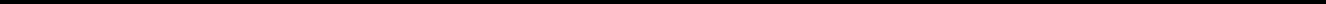
\includegraphics[width=19cm, height=5cm]{_extensions/cday/RtpPDF/footer-line.png}%
      }
    }%
  }
}
\setlength{\footskip}{35pt}


\usepackage{titlesec}
\titleformat{\subsubsection}
  {\normalfont\bfseries}{\thesubsubsection.}{1em}{}
\setcounter{secnumdepth}{4}

%% Style the chapter/section fonts
\chapterfont{\color{dark}\fontsize{28}{15}\selectfont}
\sectionfont{\color{light}\fontsize{20}{15}\selectfont}
\subsectionfont{\color{light}\fontsize{16}{15}\selectfont}
\subsubsectionfont{\color{light}\fontsize{13}{15}\selectfont}

% Redefine \@makechapterhead to format chapter titles
\makeatletter
\renewcommand{\@makechapterhead}[1]{%
  \vspace*{-30pt}% Adjust the vertical spacing before the chapter title
  {\parindent \z@ \raggedright \normalfont
    \ifnum \c@secnumdepth >\m@ne
      \if@mainmatter
        \color{dark}\sffamily\Huge\bfseries \thechapter\hspace{0.5em}% Add two spaces after chapter number
      \fi
    \fi
    \interlinepenalty\@M
    \sffamily\Huge \bfseries #1\par % Chapter title formatting
    \nobreak
    \vskip 40\p@ % Adjust the vertical spacing after the chapter title
  }}
\makeatother

\makeatletter
\renewcommand{\maketitle}{\bgroup\setlength{\parindent}{0pt}
  \vspace*{\baselineskip}
  \vspace*{\baselineskip}
  \vspace*{\baselineskip}
  \hspace*{2.3cm} {\sffamily\Huge\textbf{\MakeUppercase{\@title}}} \newline \newline
  \hspace*{2.3cm} \@author \newline \newline
  \hspace*{2.3cm} \@date % Display the date
\egroup
}
\makeatother

%% Use custom fonts
\setsansfont{AzoSans}[
    Path=_extensions/cday/RtpPDF/AzoSans/,
    Scale=0.9,
    Extension = .ttf,
    UprightFont=*-Regular,
    BoldFont=*-Bold,
    ItalicFont=*-Italic,
]

\setmainfont{AzoSans}[
    Path=_extensions/cday/RtpPDF/AzoSans/,
    Scale=0.9,
    Extension = .ttf,
    UprightFont=*-Regular,
    BoldFont=*-Bold,
    ItalicFont=*-Italic,
]

\usepackage{enumitem}
\usepackage{graphicx}

\renewcommand{\labelitemi}{
\includegraphics[width=0.5cm]{_extensions/cday/RtpPDF/rtp_bullet2.png}}
\renewcommand{\labelitemii}{
\includegraphics[width=0.5cm]{_extensions/cday/RtpPDF/rtp_bullet2.png}}
\renewcommand{\labelitemiii}{
\includegraphics[width=0.5cm]{_extensions/cday/RtpPDF/rtp_bullet2.png}}
\renewcommand{\labelitemiv}{
\includegraphics[width=0.5cm]{_extensions/cday/RtpPDF/rtp_bullet2.png}}

\KOMAoption{captions}{tableheading}
\makeatletter
\makeatother
\makeatletter
\@ifpackageloaded{bookmark}{}{\usepackage{bookmark}}
\makeatother
\makeatletter
\@ifpackageloaded{caption}{}{\usepackage{caption}}
\AtBeginDocument{%
\ifdefined\contentsname
  \renewcommand*\contentsname{Table of contents}
\else
  \newcommand\contentsname{Table of contents}
\fi
\ifdefined\listfigurename
  \renewcommand*\listfigurename{List of Figures}
\else
  \newcommand\listfigurename{List of Figures}
\fi
\ifdefined\listtablename
  \renewcommand*\listtablename{List of Tables}
\else
  \newcommand\listtablename{List of Tables}
\fi
\ifdefined\figurename
  \renewcommand*\figurename{Figure}
\else
  \newcommand\figurename{Figure}
\fi
\ifdefined\tablename
  \renewcommand*\tablename{Table}
\else
  \newcommand\tablename{Table}
\fi
}
\@ifpackageloaded{float}{}{\usepackage{float}}
\floatstyle{ruled}
\@ifundefined{c@chapter}{\newfloat{codelisting}{h}{lop}}{\newfloat{codelisting}{h}{lop}[chapter]}
\floatname{codelisting}{Listing}
\newcommand*\listoflistings{\listof{codelisting}{List of Listings}}
\makeatother
\makeatletter
\@ifpackageloaded{caption}{}{\usepackage{caption}}
\@ifpackageloaded{subcaption}{}{\usepackage{subcaption}}
\makeatother
\makeatletter
\@ifpackageloaded{tcolorbox}{}{\usepackage[skins,breakable]{tcolorbox}}
\makeatother
\makeatletter
\@ifundefined{shadecolor}{\definecolor{shadecolor}{rgb}{.97, .97, .97}}
\makeatother
\makeatletter
\@ifundefined{codebgcolor}{\definecolor{codebgcolor}{named}{light}}
\makeatother
\makeatletter
\makeatother
\ifLuaTeX
  \usepackage{selnolig}  % disable illegal ligatures
\fi
\IfFileExists{bookmark.sty}{\usepackage{bookmark}}{\usepackage{hyperref}}
\IfFileExists{xurl.sty}{\usepackage{xurl}}{} % add URL line breaks if available
\urlstyle{same} % disable monospaced font for URLs
\hypersetup{
  pdftitle={Validation Report - Version 9.0.0},
  pdfauthor={WFRC / MAG},
  colorlinks=true,
  linkcolor={highlight},
  filecolor={Maroon},
  citecolor={Blue},
  urlcolor={highlight},
  pdfcreator={LaTeX via pandoc}}

\title{Validation Report - Version 9.0.0}
\author{WFRC / MAG}
\date{August 1, 2023}

\begin{document}
\maketitle
\pagestyle{mystyle}

\ifdefined\Shaded\renewenvironment{Shaded}{\begin{tcolorbox}[sharp corners, boxrule=0pt, colback={codebgcolor}, breakable, frame hidden, borderline west={3pt}{0pt}{shadecolor}, enhanced]}{\end{tcolorbox}}\fi

\renewcommand*\contentsname{Table of contents}
{
\hypersetup{linkcolor=}
\setcounter{tocdepth}{2}
\tableofcontents
}
\listoffigures
\listoftables
\bookmarksetup{startatroot}

\hypertarget{documentation}{%
\chapter{Documentation}\label{documentation}}

Documentation of the Wasatch Front Travel Demand Model (WF TDM) has been
separated into three documents:

\begin{itemize}
\tightlist
\item
  What's New Report -- describes the changes made to the WF TDM since
  the last model release
\item
  Validation Report -- provides the base year validation of the current
  version of the WF TDM, as well as a reasonableness check of the model
  as a forecasting tool
\item
  Model Process Report -- provides an overview of the model, a summary
  of the model's input data sets, and an outline of the model's primary
  steps and logic
\end{itemize}

These reports will be available as PDF documents in the ``\_Notes''
folder in the WF TDM's root directory. However, it is expected that the
primary means of accessing the model's documentation will be online at
the following links:

\begin{itemize}
\tightlist
\item
  \href{https://wfrc.org/wftdm-docs/v9x/v900/whats-new/1-genparams.html}{What's
  New}
\item
  \href{https://wfrc.org/wftdm-docs/v9x/v900/validation/3-distribute.html}{Validation
  Report}
\item
  Model Process Report (in progress)
\item
  Previous Versions (in progress)
\end{itemize}

\bookmarksetup{startatroot}

\hypertarget{household-disaggregation-and-auto-ownership}{%
\chapter{Household Disaggregation and Auto
Ownership}\label{household-disaggregation-and-auto-ownership}}

\hypertarget{life-cycle}{%
\section{Life Cycle}\label{life-cycle}}

The validation of the Life Cycle model includes the comparison of model
output to observed data for the following categories:

\begin{itemize}
\tightlist
\item
  Population by Age Group and County
\item
  Population by Life Cycle
\item
  Households by Life Cycle
\end{itemize}

For Population by Age Group and County model results are compared to
observed data as represented by the Kem C. Gardner Policy Institute
(GPI) control totals. Population by Life Cycle and Households by Life
Cycle are compared to the Utah Household Travel Survey.

Life Cycle comparisons are summarized by the following three life cycle
categories:

\begin{itemize}
\tightlist
\item
  Life Cycle 1 -- households with no children and no seniors
\item
  Life Cycle 2 -- households with children and no seniors
\item
  Life Cycle 3 -- households with seniors (may have children)
\end{itemize}

\hypertarget{population-by-age-group-and-county}{%
\section{Population by Age Group and
County}\label{population-by-age-group-and-county}}

The 2020 model base year population by county and Age Group was compared
to the 2020 GPI county-level population by Age Group, shown in
Figure~\ref{fig-pdf-age-comp}. The model's estimate of the population in
each Age Group mirrors the GPI county-level projections.

\begin{figure}[H]

{\centering 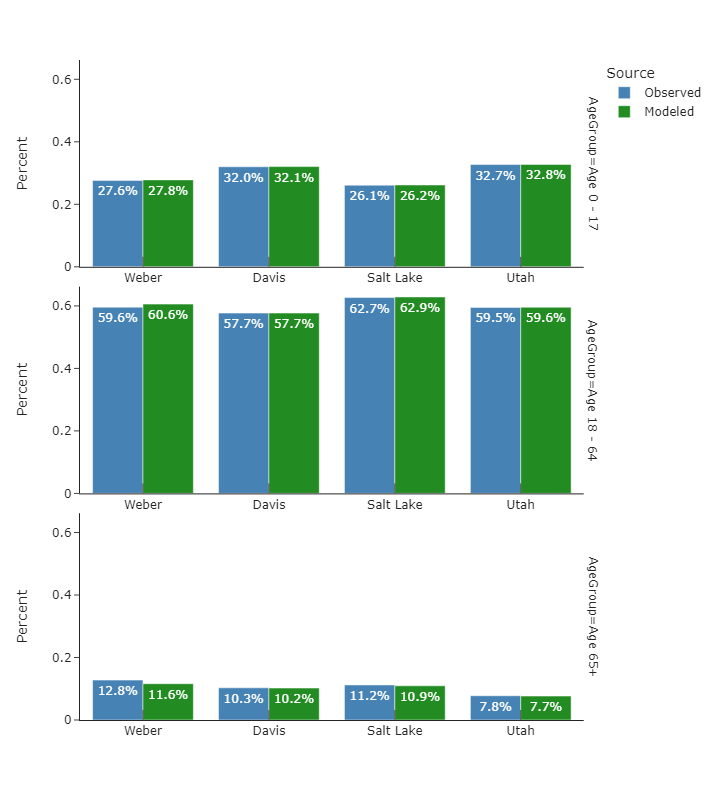
\includegraphics{v9x/v900/validation/_pictures/1-plot3.png}

}

\caption{\label{fig-pdf-age-comp}2020 Model vs.~2020 GPI -- \%
Population by Age Group and County.}

\end{figure}

\hypertarget{population-by-life-cycle}{%
\section{Population by Life Cycle}\label{population-by-life-cycle}}

The shares of the modeled 2019 base year population by Life Cycle were
compared to the 2012 Household Survey at the county level. The model's
estimate of population by Life Cycle category seemed reasonable at this
level of geography with all modeled comparison points falling within 4\%
of the observed data.

\begin{figure}[H]

{\centering 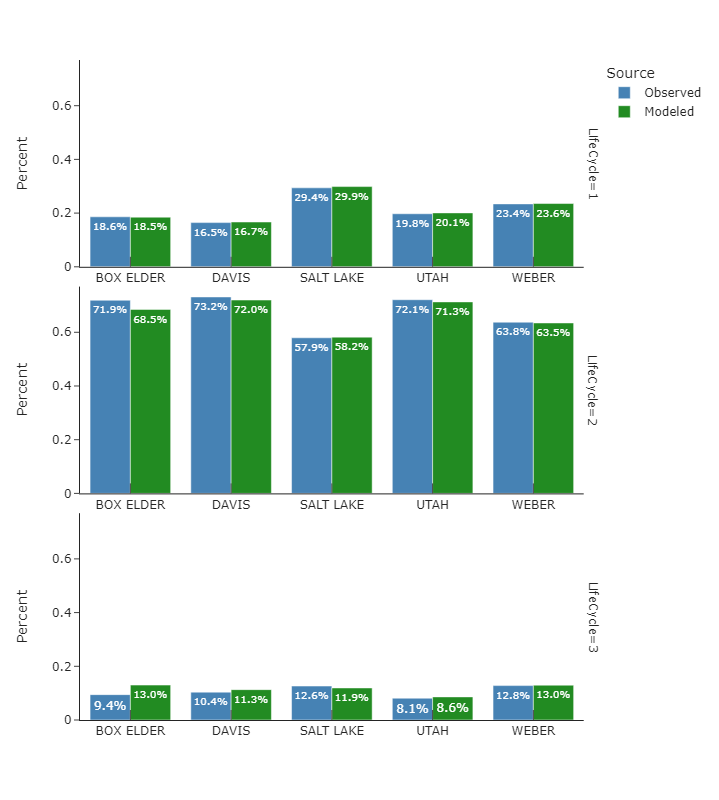
\includegraphics{v9x/v900/validation/_pictures/1-plot4.png}

}

\caption{\label{fig-pdf-lc-pop}2019 Model vs.~2012 Household Survey --
\% Population by Life Cycle and County.}

\end{figure}

\hypertarget{households-by-life-cycle}{%
\section{Households by Life Cycle}\label{households-by-life-cycle}}

The shares of the modeled 2019 base year households by Life Cycle were
compared to the 2012 Household Survey at the county level. The model's
estimate of households by Life Cycle category seemed reasonable at this
level of geography with all modeled comparison points falling within
1.5\% of the observed data.

\begin{figure}[H]

{\centering 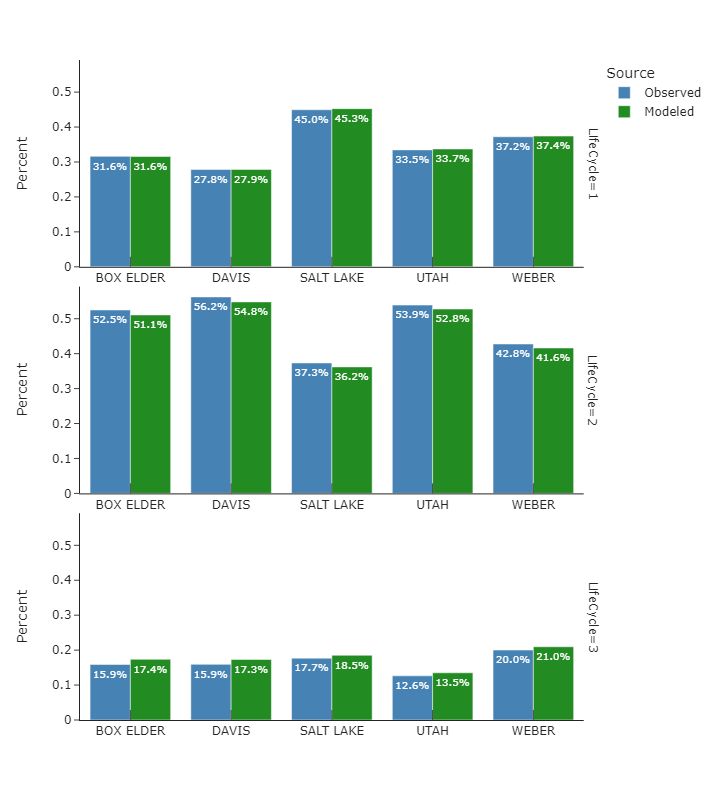
\includegraphics{v9x/v900/validation/_pictures/1-plot5.png}

}

\caption{\label{fig-pdf-lc-hh}2019 Model vs.~2012 Household Survey -- \%
Households by Life Cycle and County.}

\end{figure}

\hypertarget{household-disaggregation}{%
\section{Household Disaggregation}\label{household-disaggregation}}

The Household Disaggregation was validated to the following measures:

\begin{itemize}
\tightlist
\item
  Household Size
\item
  Income
\item
  Number of Workers
\end{itemize}

\hypertarget{household-size}{%
\subsection{Household Size}\label{household-size}}

The shares of the modeled 2015 base year households by Household Size
category were validated to 2010 Census and 2016 ACS data at the county
level. The model's estimate of households by each of the six Household
Size category matches within about 2\% of the observed data for all
counties.

???Update to use 2019 Model???\textgreater\textgreater{}

\begin{figure}[H]

{\centering 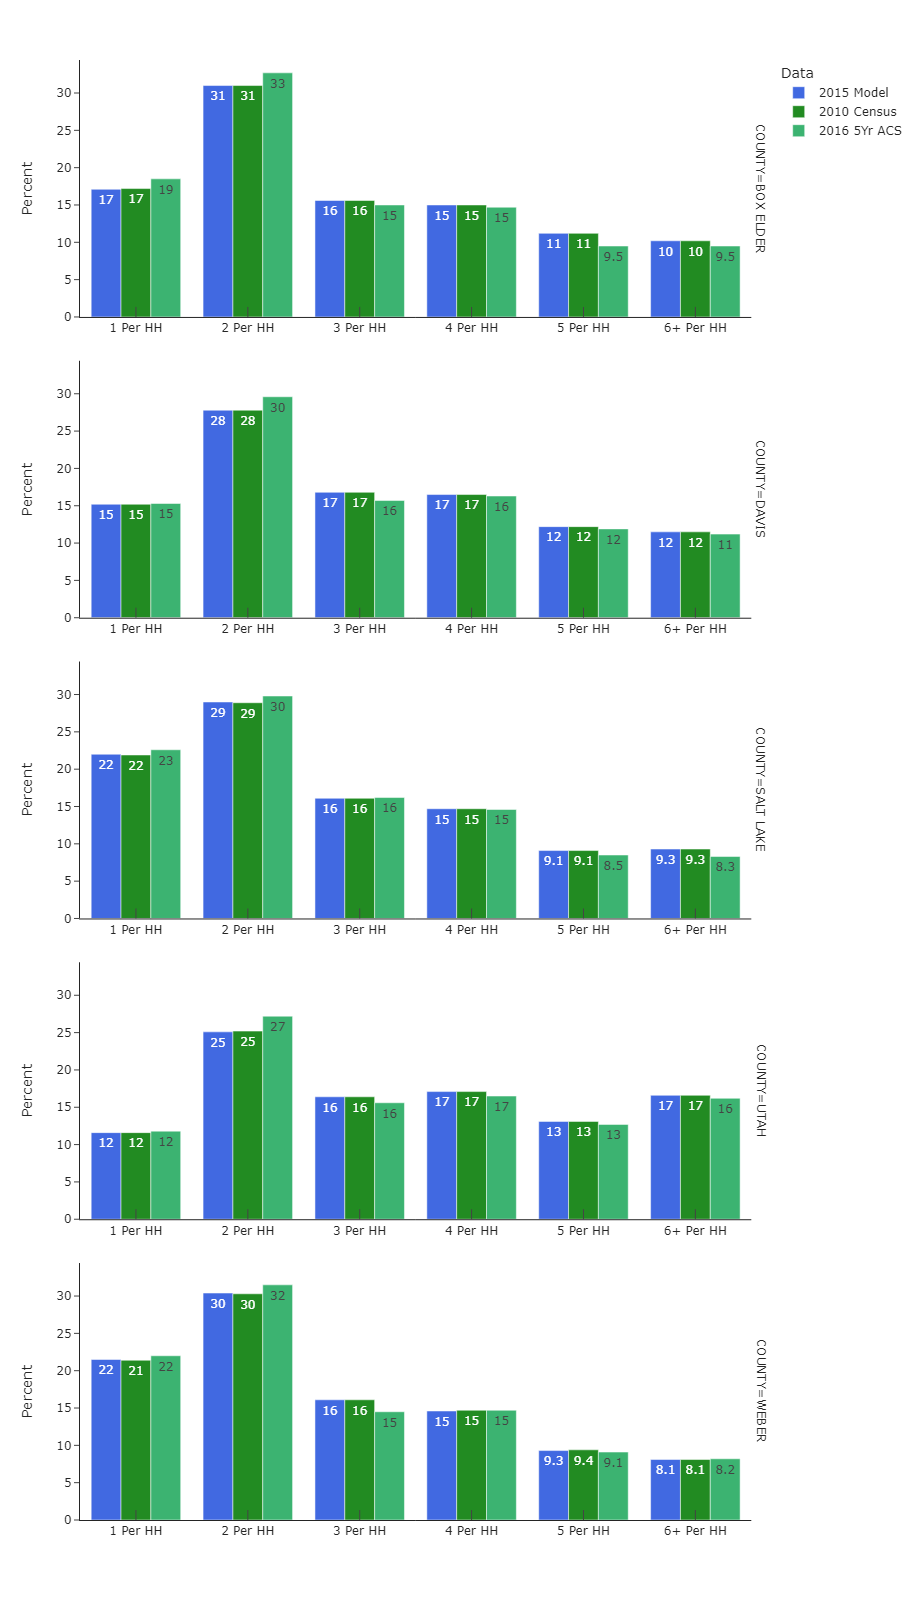
\includegraphics[width=\textwidth,height=0.9\textheight]{v9x/v900/validation/_pictures/2-plot7.png}

}

\caption{\label{fig-pdf-hh-modobs}2015 Model vs.~2010 Census \& 2016 ACS
-- \% Households by Household Size.}

\end{figure}

\hypertarget{income}{%
\subsection{Income}\label{income}}

???UPDATE -- maybe from validation in this location: A:\textbackslash1 -
TDM\textbackslash2 - Estimate Param\textbackslash1 - HHDisag\_AutoOwn???

\begin{itemize}
\tightlist
\item
  Income Gruops (Income Levels) in 2016 dollars:

  \begin{itemize}
  \tightlist
  \item
    1: \$0 to 35,000 (Low)
  \item
    2: \$35,000 to 60,000 (High)
  \item
    3: \$60,000 to 100,000 (High)
  \item
    4: \$100,000 and above (High)
  \end{itemize}
\end{itemize}

\hypertarget{worker}{%
\subsection{Worker}\label{worker}}

\begin{itemize}
\tightlist
\item
  Worker Groups: 0, 1, 2, 3+ workers per household
\end{itemize}

???UPDATE -- maybe from validation in this location: A:\textbackslash1 -
TDM\textbackslash2 - Estimate Param\textbackslash1 - HHDisag\_AutoOwn???

\hypertarget{auto-ownership}{%
\section{Auto Ownership}\label{auto-ownership}}

???Which validation charts should I add???

\bookmarksetup{startatroot}

\hypertarget{trip-generation}{%
\chapter{Trip Generation}\label{trip-generation}}

\hypertarget{validation-results}{%
\section{Validation Results}\label{validation-results}}

The validation results for the Trip Generation portion of the model are
shown in this section.

???All the 2012 Household Survey results are scaled to the 2010
Census.-- is the scaled to the 2020 census now???

\begin{figure}[H]

{\centering 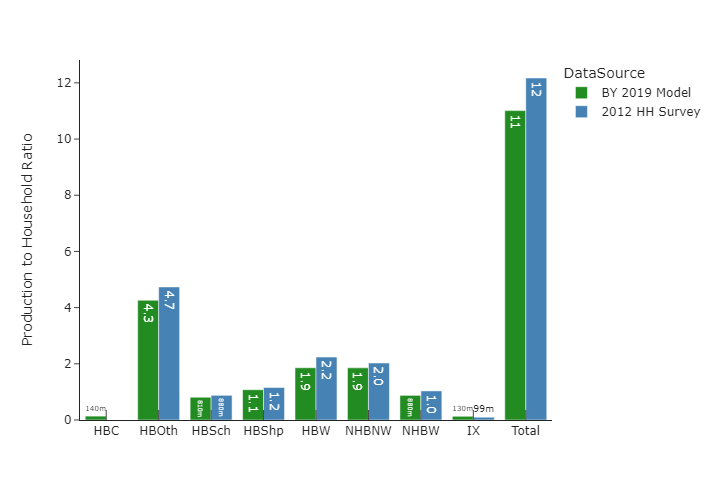
\includegraphics{v9x/v900/validation/_pictures/4-plot1.png}

}

\caption{\label{fig-pdf-prod-hh}Productions to Households Ratios --
Total Trip Ends (II + IX).}

\end{figure}

\begin{figure}[H]

{\centering 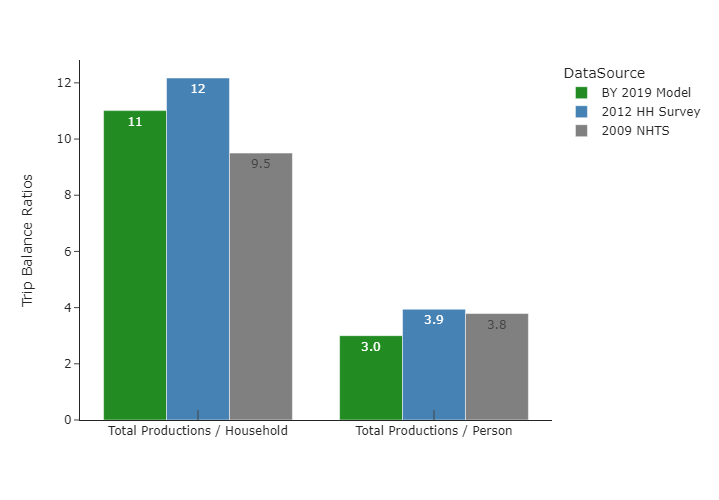
\includegraphics{v9x/v900/validation/_pictures/4-plot2.png}

}

\caption{\label{fig-pdf-ptrip-valid}Total Trip Validation.}

\end{figure}

\begin{figure}[H]

{\centering 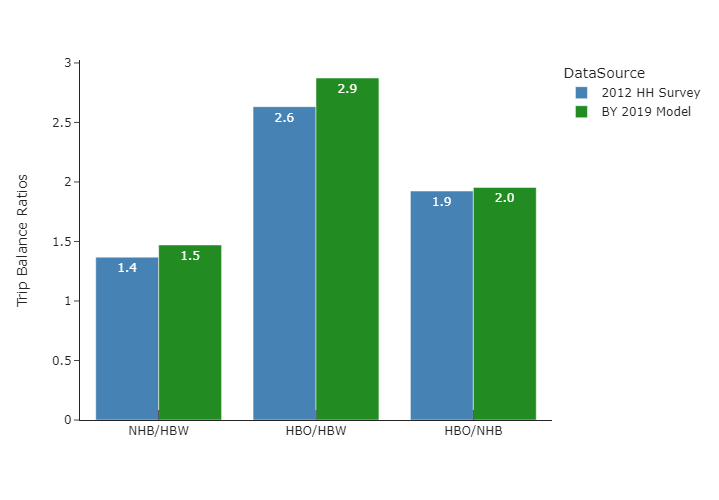
\includegraphics{v9x/v900/validation/_pictures/4-plot3.png}

}

\caption{\label{fig-pdf-prod-prod}Trip Balance Ratios.}

\end{figure}

\bookmarksetup{startatroot}

\hypertarget{trip-distribution}{%
\chapter{Trip Distribution}\label{trip-distribution}}

The validation for the Trip Distribution are shown in this section. The
observed data comes from the 2012 Household Survey.

The model and observed data are compared below by trip purpose for the
following variables:

\begin{itemize}
\tightlist
\item
  Trip Generalized Cost
\item
  Distance
\item
  Time
\end{itemize}

\begin{figure}[H]

{\centering 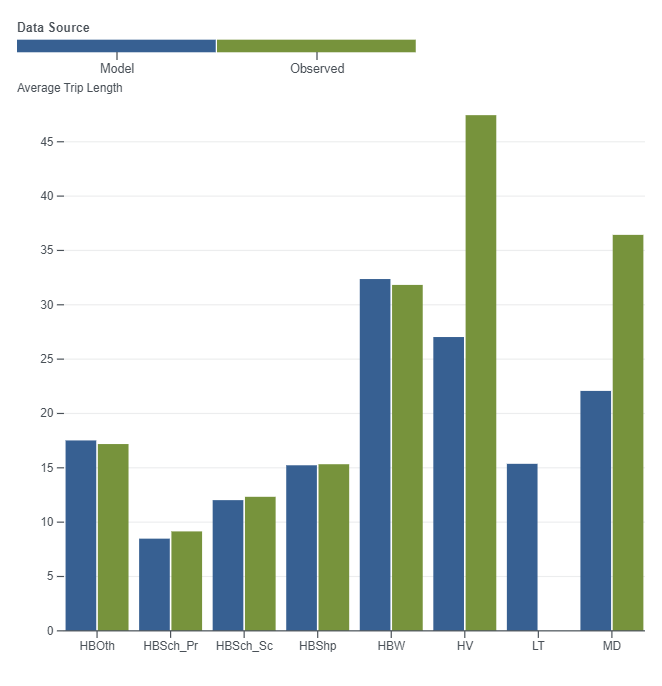
\includegraphics[width=\textwidth,height=0.4\textheight]{v9x/v900/validation/_pictures/5-plot1.png}

}

\caption{\label{fig-pdf-gc-purp}Average Trip Length for Generalized Cost
for Main Purposes.}

\end{figure}

\begin{figure}[H]

{\centering 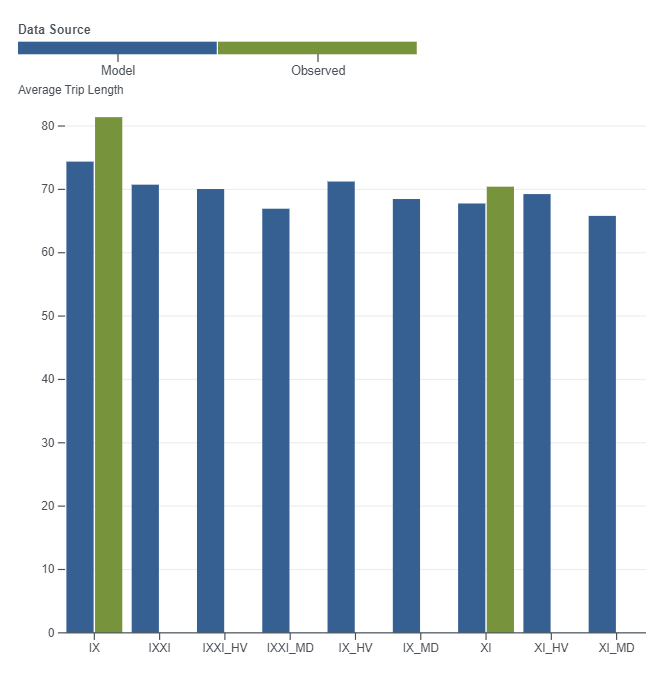
\includegraphics[width=\textwidth,height=0.4\textheight]{v9x/v900/validation/_pictures/5-plot2.png}

}

\caption{\label{fig-pdf-gc-ext}Average Trip Length for Generalized Cost
for External Forces.}

\end{figure}

\begin{figure}[H]

{\centering 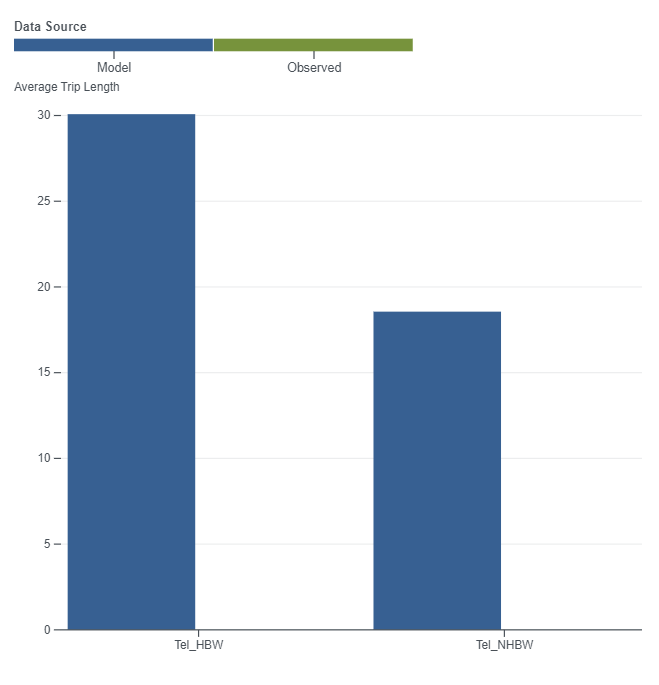
\includegraphics[width=\textwidth,height=0.4\textheight]{v9x/v900/validation/_pictures/5-plot3.png}

}

\caption{\label{fig-pdf-cg-tele}Average Trip Length for Generalized Cost
for Telecommuting.}

\end{figure}

\begin{figure}[H]

{\centering 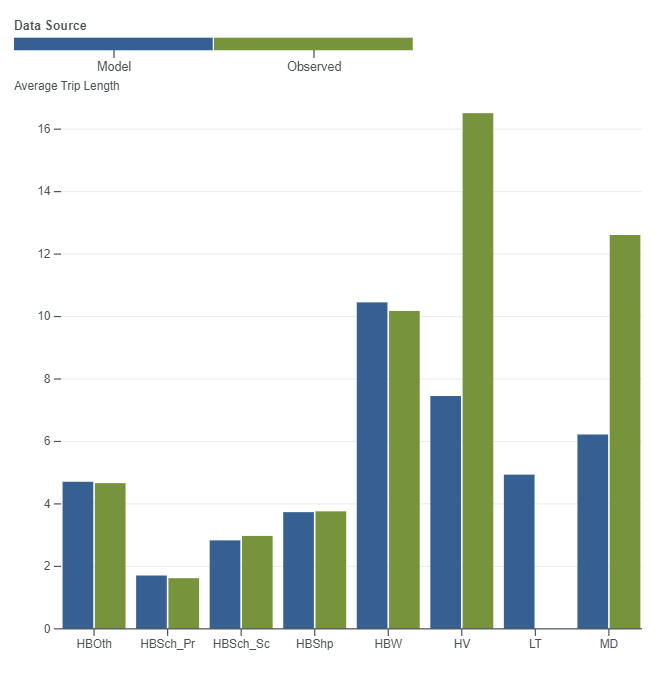
\includegraphics[width=\textwidth,height=0.4\textheight]{v9x/v900/validation/_pictures/5-plot4.png}

}

\caption{\label{fig-pdf-dist-purp}Average Trip Length for Distance for
Main Purposes.}

\end{figure}

\begin{figure}[H]

{\centering 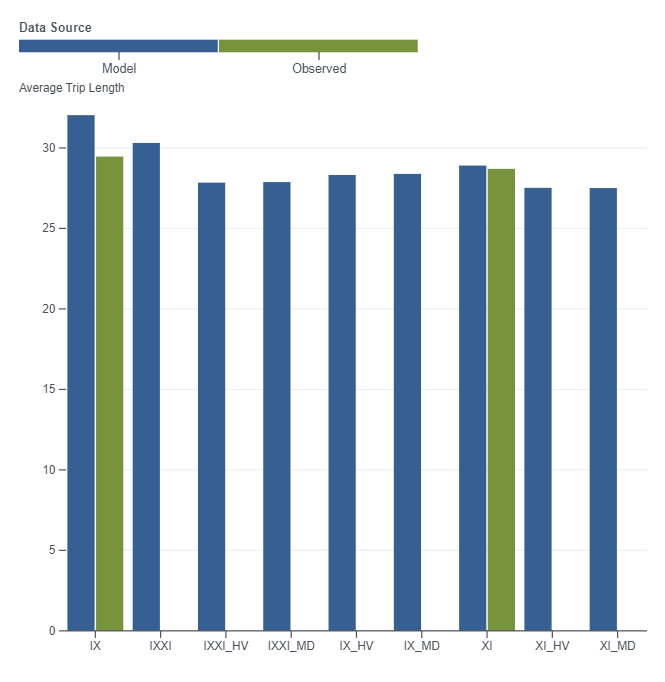
\includegraphics[width=\textwidth,height=0.4\textheight]{v9x/v900/validation/_pictures/5-plot5.png}

}

\caption{\label{fig-pdf-dist-ext}Average Trip Length for Distance for
External Forces.}

\end{figure}

\begin{figure}[H]

{\centering 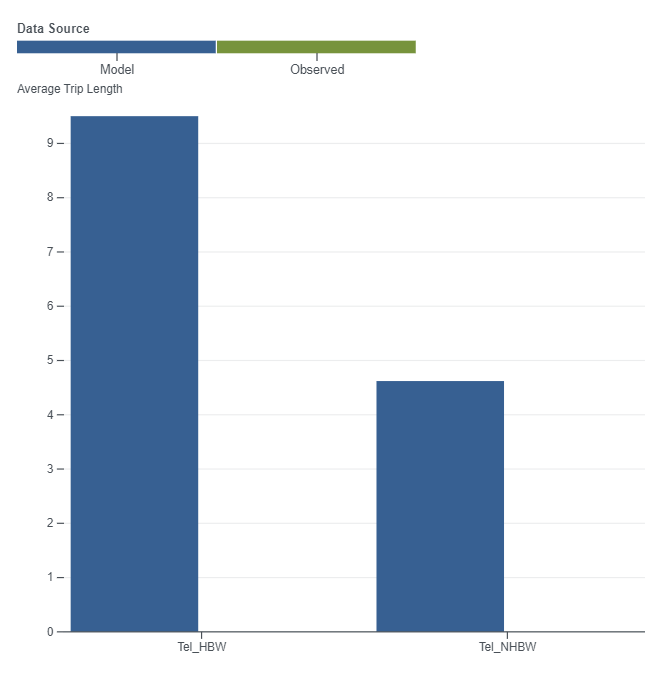
\includegraphics[width=\textwidth,height=0.4\textheight]{v9x/v900/validation/_pictures/5-plot6.png}

}

\caption{\label{fig-pdf-dist-tele}Average Trip Length for Distance for
Telecommuting.}

\end{figure}

\begin{figure}[H]

{\centering 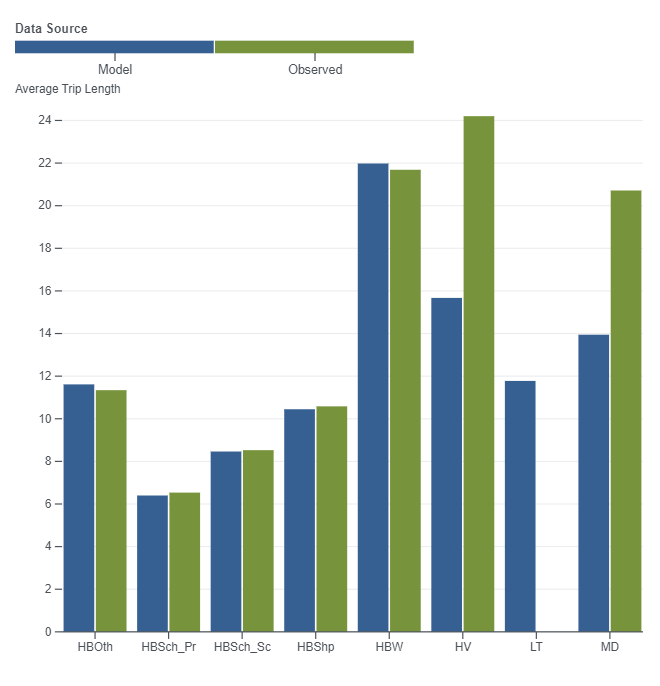
\includegraphics[width=\textwidth,height=0.4\textheight]{v9x/v900/validation/_pictures/5-plot7.png}

}

\caption{\label{fig-pdf-time-purp}Average Trip Length for Time for Main
Purposes.}

\end{figure}

\begin{figure}[H]

{\centering 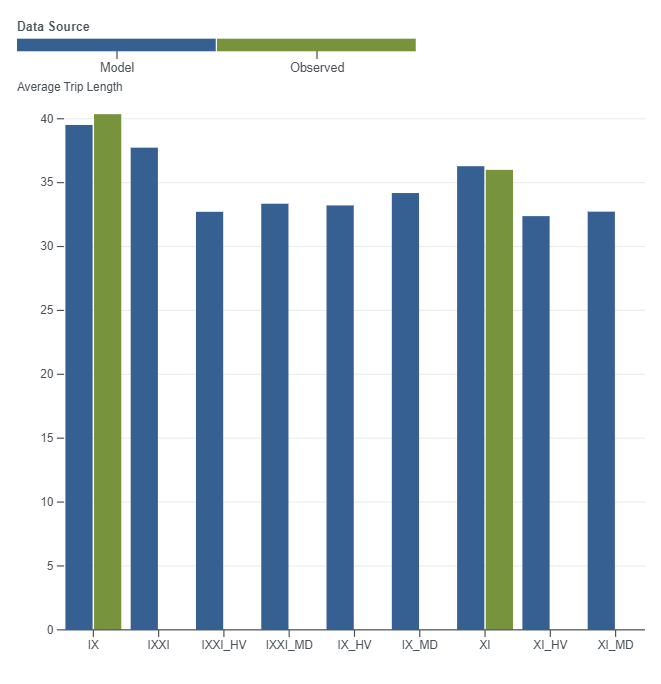
\includegraphics[width=\textwidth,height=0.4\textheight]{v9x/v900/validation/_pictures/5-plot8.png}

}

\caption{\label{fig-pdf-time-ext}Average Trip Length for Time for
External Forces.}

\end{figure}

\begin{figure}[H]

{\centering 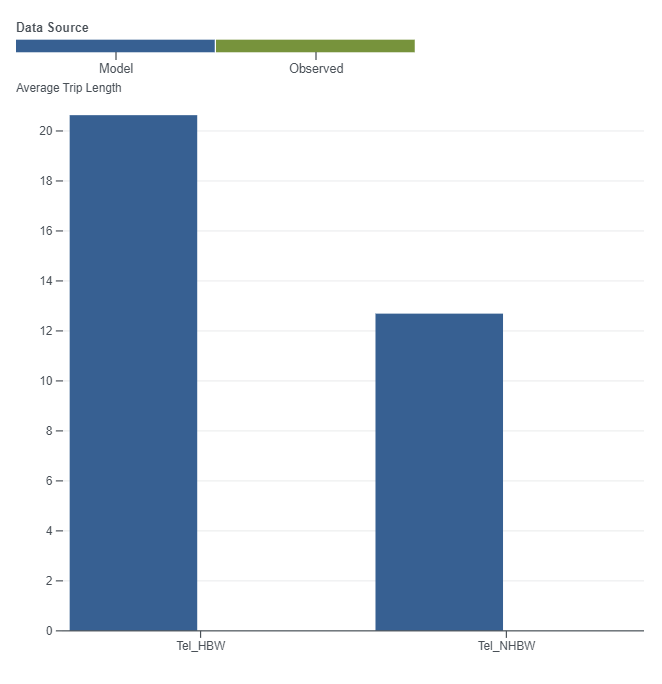
\includegraphics[width=\textwidth,height=0.4\textheight]{v9x/v900/validation/_pictures/5-plot9.png}

}

\caption{\label{fig-pdf-time-tele}Average Trip Length for Time for
Telecommuting.}

\end{figure}

\bookmarksetup{startatroot}

\hypertarget{mode-choice}{%
\chapter{Mode Choice}\label{mode-choice}}

The validation results for the Mode Choice portion of the model are
shown in this section. Mode Choice was validated against the Utah
Transit Authority 2019 On-Board Survey as well as the 2012 Household
Travel Survey. Validation is summarized by the following categories:

\begin{itemize}
\tightlist
\item
  Transit Trips and Boardings
\item
  Mode Share
\end{itemize}

\begin{verbatim}
<IPython.core.display.HTML object>
\end{verbatim}

\begin{verbatim}
<IPython.core.display.HTML object>
\end{verbatim}

\begin{verbatim}
<IPython.core.display.HTML object>
\end{verbatim}

\begin{verbatim}
<IPython.core.display.HTML object>
\end{verbatim}

\begin{verbatim}
<IPython.core.display.HTML object>
\end{verbatim}

\begin{verbatim}
<IPython.core.display.HTML object>
\end{verbatim}

\begin{verbatim}
<IPython.core.display.HTML object>
\end{verbatim}

\begin{verbatim}
<IPython.core.display.HTML object>
\end{verbatim}

\begin{verbatim}
<IPython.core.display.HTML object>
\end{verbatim}

\begin{verbatim}
<IPython.core.display.HTML object>
\end{verbatim}

\begin{verbatim}
<IPython.core.display.HTML object>
\end{verbatim}

\begin{verbatim}
<IPython.core.display.HTML object>
\end{verbatim}

\hypertarget{transit-trips-and-boardings}{%
\section{Transit Trips and
Boardings}\label{transit-trips-and-boardings}}

The validation of daily transit trips and boardings is shown through the
comparison of model and observed data by mode. The model was validated
by the following measures:

\begin{itemize}
\tightlist
\item
  Trips by Hierarchical Mode
\item
  Boardings by Hierarchical Mode
\item
  Transfer Ratio by Hierarchical Mode
\item
  Boardings by Surveyed Mode (for comparison only)
\end{itemize}

The three hierarchical mode measures are summarized by the highest
hierarchy mode in a given trip with local bus being the lowest on the
hierarchy and commuter rail being the highest. For example, if a trip
uses Local Bus and then transfers to LRT, the trip is stored as a LRT
trip. \emph{Trips by Hierarchical Mode} represent each trip as a single
number, regardless of the number of transfer or different modes that
were used on a trip.

\emph{Boardings by Hierarchical Mode} represent each boarding separately
but summarized at the highest hierarchical mode of the trip. For
example, for one transfer from Local Bus to LRT there are two boardings,
one on each mode, but they are both stored in the highest hierarchal
mode of LRT. The Transfer Ratio by \emph{Hierarchical Mode} is the ratio
between boardings and trips for any given mode.

The final measure \emph{Boardings by Surveyed Mode} represents the total
boardings on each mode individually. They are not summarize at the
highest hierarchical mode of the trip but rather at the mode on which
the boarding actually occurred. For example, the Local Bus to LRT trip
mentioned previously would be summarized in this measure as one boarding
on Local Bus and one boarding one LRT. This measure is for comparison
use only, since the structure of the Mode Choice model does not consider
this measure during calibration.

The total number of boardings are the same between hierarchical mode and
surveyed mode, but depending on the make-up of the trips, there totals
by mode will vary.

The model data for hierarchical mode measures is taken from the shares
reports \texttt{v9\_SE19\_Net19\_RegionShares\_Pk.csv} and
\texttt{v9\_SE19\_Net19\_RegionShares\_Ok.csv}. The model data for the
surveyed mode comparison is taken from
\texttt{\_v9\_SE19\_Net19\_1\_PA\_Route.dbf}.

The interactive \textbf{?@fig-mc-boardings} allows for the visual
comparison of model and observed values for each \emph{Transit Trips and
Boardings} category.

\begin{Shaded}
\begin{Highlighting}[]
\NormalTok{html\textasciigrave{}\textless{}br/\textgreater{}\textasciigrave{}}
\NormalTok{viewof bPlotSelect = Inputs.select(new Map([[\textquotesingle{}Trips by Hierarchical Mode\textquotesingle{}, \textquotesingle{}Trips by Hierarchical Mode\textquotesingle{}], [\textquotesingle{}Boardings by Hierarchical Mode\textquotesingle{}, \textquotesingle{}Boardings by Hierarchical Mode\textquotesingle{}], [\textquotesingle{}Transfer Ratio by Hierarchical Mode\textquotesingle{},\textquotesingle{}Transfer Ratio\textquotesingle{}], [\textquotesingle{}Boardings by Mode Surveyed\textquotesingle{},\textquotesingle{}Boardings by Mode Surveyed\textquotesingle{}]]), \{value: nameGroup, label: "Category"\})}
\NormalTok{viewof metric = Inputs.radio(new Map([["Difference", "Difference"], ["\% Difference", "\% Difference"]]), \{value: "Difference", label: "View:"\})}

\NormalTok{dataBLC = transpose(boardChart)}
\NormalTok{filtered\_bDataC = dataBLC.filter(function(dataBLC) \{}
\NormalTok{    return bPlotSelect == dataBLC.Title \&\&}
\NormalTok{           "Value" == dataBLC.View;}
\NormalTok{\})}
\NormalTok{dataBTT = transpose(boardTable)}
\NormalTok{filtered\_bDataT = dataBTT.filter(function(dataBTT) \{}
\NormalTok{    return bPlotSelect == dataBTT.Title;}
\NormalTok{\})}
\end{Highlighting}
\end{Shaded}

\begin{Shaded}
\begin{Highlighting}[]
\NormalTok{html\textasciigrave{}}
\NormalTok{\textless{}br/\textgreater{}}
\NormalTok{\textless{}table\textgreater{}}
\NormalTok{    \textless{}thead\textgreater{}}
\NormalTok{    \textless{}tr\textgreater{}}
\NormalTok{        $\{["Mode", "Model", "Observed", "Difference", "\% Difference"].map((d, i) =\textgreater{} \{}
\NormalTok{            const widths = [\textquotesingle{}90px\textquotesingle{}, \textquotesingle{}60px\textquotesingle{}, \textquotesingle{}70px\textquotesingle{}, \textquotesingle{}75px\textquotesingle{}, \textquotesingle{}90px\textquotesingle{}]; // Define the widths}
\NormalTok{            return html\textasciigrave{}\textless{}th style=\textquotesingle{}text{-}align: $\{i === 0 ? "left" : "right"\}; padding: 5px; width: $\{widths[i]\};\textquotesingle{}\textgreater{}$\{d\}\textless{}/th\textgreater{}\textasciigrave{};}
\NormalTok{        \})\}}
\NormalTok{    \textless{}/tr\textgreater{}}
\NormalTok{    \textless{}/thead\textgreater{}}
\NormalTok{    \textless{}tbody\textgreater{}}
\NormalTok{        $\{filtered\_bDataT.map(row =\textgreater{} \{}
\NormalTok{            const isBold = row[\textquotesingle{}Mode\textquotesingle{}] === \textquotesingle{}Total\textquotesingle{};}
\NormalTok{            return html\textasciigrave{}\textless{}tr style=\textquotesingle{}border{-}bottom: 1px solid lightgrey;\textquotesingle{}\textgreater{}}
\NormalTok{                $\{["Mode", "Model", "Observed", "Difference", "\% Difference"].map((d, i) =\textgreater{} \{}
\NormalTok{                    const widths = [\textquotesingle{}90px\textquotesingle{}, \textquotesingle{}60px\textquotesingle{}, \textquotesingle{}70px\textquotesingle{}, \textquotesingle{}75px\textquotesingle{}, \textquotesingle{}90px\textquotesingle{}]; // Define the widths}
\NormalTok{                    return html\textasciigrave{}\textless{}td style=\textquotesingle{}text{-}align: $\{i === 0 ? "left" : "right"\}; padding: 5px; width: $\{widths[i]\}; font{-}weight: $\{isBold ? \textquotesingle{}bold\textquotesingle{} : \textquotesingle{}normal\textquotesingle{}\};\textquotesingle{}\textgreater{}$\{row[d]\}\textless{}/td\textgreater{}\textasciigrave{};}
\NormalTok{                \})\}}
\NormalTok{            \textless{}/tr\textgreater{}\textasciigrave{};}
\NormalTok{        \})\}}
\NormalTok{    \textless{}/tbody\textgreater{}}
\NormalTok{\textless{}/table\textgreater{}\textasciigrave{}}
\end{Highlighting}
\end{Shaded}

\begin{Shaded}
\begin{Highlighting}[]
\NormalTok{key2 = Legend(bChart.scales.color, \{title: "Data Source"\})}

\NormalTok{bChart = GroupedBarChart(filtered\_bDataC, \{}
\NormalTok{    x: d =\textgreater{} d.Mode,}
\NormalTok{    y: d =\textgreater{} d.ViewValue,}
\NormalTok{    z: d =\textgreater{} d.DataSource,}
\NormalTok{    xDomain: [\textquotesingle{}Local Bus\textquotesingle{}, \textquotesingle{}Core Bus\textquotesingle{}, \textquotesingle{}Express Bus\textquotesingle{}, \textquotesingle{}BRT\textquotesingle{}, \textquotesingle{}LRT\textquotesingle{}, \textquotesingle{}CRT\textquotesingle{}],}
\NormalTok{    yLabel: "Value",}
\NormalTok{    zDomain: [\textquotesingle{}Model\textquotesingle{},\textquotesingle{}Observed\textquotesingle{}],}
\NormalTok{    width: 500,}
\NormalTok{    height: 225,}
\NormalTok{    colors: ["\#376092", "\#77933c"]}
\NormalTok{\})}
\end{Highlighting}
\end{Shaded}

\begin{Shaded}
\begin{Highlighting}[]
\NormalTok{filtered\_bData2 = dataBLC.filter(function(dataBLC) \{}
\NormalTok{    return bPlotSelect == dataBLC.Title  \&\&}
\NormalTok{           metric == dataBLC.View;}
\NormalTok{\})}

\NormalTok{//https://observablehq.com/@d3/diverging{-}bar{-}chart}
\NormalTok{import \{DivergingBarChart\} from "@d3/diverging{-}bar{-}chart"}

\NormalTok{html\textasciigrave{}\textless{}br/\textgreater{}\textasciigrave{}}
\NormalTok{chart3 = DivergingBarChart(filtered\_bData2, \{}
\NormalTok{    x: d =\textgreater{} d.ViewValue,}
\NormalTok{    y: d =\textgreater{} d.Mode,}
\NormalTok{    xFormat: metric === "Difference" ? "+,d" : "+\%",}
\NormalTok{    xLabel: "Model vs Observed Differences",}
\NormalTok{    height: 200,}
\NormalTok{    colors: d3.schemeRdBu[3]}
\NormalTok{\})}
\end{Highlighting}
\end{Shaded}

\begin{Shaded}
\begin{Highlighting}[]
\NormalTok{//|label: fig{-}mc{-}boardings}
\NormalTok{//|fig{-}cap: Transit Trips and Boardings Model vs Observed Comparison}
\NormalTok{tbEmptyCell = 1}
\end{Highlighting}
\end{Shaded}

\begin{Shaded}
\begin{Highlighting}[]
\NormalTok{html\textasciigrave{}\textless{}br/\textgreater{}\textasciigrave{}}
\end{Highlighting}
\end{Shaded}

When considering \emph{Trips by Hierarchical Mode}, the calibration
routine of the model results in the total number of transit trips in the
model being very close to the observed. For this model the model trips
are only 0.2\% higher than observed for the total number of trips. By
mode the differences are within reasonable ranges for the higher trip
modes. For example, LRT is only 0.1\% high and CRT is only 0.8\% low.

Due to the very low number of trips for Core Bus and Express Bus, their
differences are acceptable. Currently, Core Bus for example has only one
route. In future phases of the RTP, additional Core Bus service is
planned. While further calibration could have brought the Core Bus
validation more in line with observed, over-calibrating the model was
not desired.

\emph{Boardings by Hierarchical Mode} show a similar pattern. Overall
boardings are only 1.9\% lower in model compared to observed, and the
modes Local Bus, LRT, and CRT all within 5\%. Core Bus is again the
furthest away, but it also is a single route with lower number of
boardings as compared to the higher boarding modes.

The \emph{Transfer Ratio by Hierarchical Mode} shows the relationship
between the trips and the boardings. While the model was only slightly
higher in trips, the boardings were low. This results in a lower
transfer ratio, which is still acceptable with all values being within
about 5\%.

And for comparison, \emph{Boardings by Mode Surveyed} shows acceptable
differences. The Core Bus and Express Bus values show much larger
differences; but again given their low volumes, these are reasonable
differences.

\hypertarget{mode-share}{%
\section{Mode Share}\label{mode-share}}

Mode Share validation is shown through the comparison by groups of mode,
time period, and trip purpose. For model and observed shares, the total
percent for each combination of mode group, time period, and trip
purpose adds up to 100\%.

Mode groups compared include groupings of auto, transit, vehicle
occupancy, and transit modes. The highest nest is motorized and
non-motorized down to lower nests of individual transit modes and
transit access modes. Shares were calculated for the following mode
groupings:

\begin{itemize}
\tightlist
\item
  Motorized / Non-Motorized
\item
  Auto / Transit
\item
  Drive Alone / Shared Ride
\item
  Shared Ride \# of Occupants
\item
  Transit Mode
\item
  Transit Access Mode
\end{itemize}

Additionally, the shares were compared by the following time period
groupings:

\begin{itemize}
\tightlist
\item
  Daily
\item
  Peak
\item
  Off-peak
\end{itemize}

Finally, the shares were further compared for each of the following trip
purposes:

\begin{itemize}
\tightlist
\item
  All Purposes
\item
  Home-Based Work
\item
  Home-Based College
\item
  Home-Based Other
\item
  Non-Home Based
\end{itemize}

In the model, Home-Based College is the only trip purpose that does not
include trips in the off-peak time period. So, any trips with this
purpose in the observed data were moved to the peak time period for
comparison.

The interactive \textbf{?@fig-mode-share} allows for selecting of
different combinations to visualize the comparisons. The observed data
comes from a combination of the Household Travel Survey and the 2019
Transit On-Board Survey.

\begin{Shaded}
\begin{Highlighting}[]
\NormalTok{html\textasciigrave{}\textless{}br/\textgreater{}\textasciigrave{}}
\NormalTok{viewof plotSelect    = Inputs.select(new Map([[nameModeMnMShare,nameModeMnMShare],}
\NormalTok{                                              [nameModeATShare ,nameModeATShare ],}
\NormalTok{                                              [nameModeDAShare ,nameModeDAShare ],}
\NormalTok{                                              [nameMode23Share ,nameMode23Share ],}
\NormalTok{                                              [nameModeTransit ,nameModeTransit ],}
\NormalTok{                                              [nameModeAccess  ,nameModeAccess  ]}
\NormalTok{                                             ]), \{value: nameGroup, label: "Mode Group:"\})}
\NormalTok{viewof periodSelect  = Inputs.select(new Map([[\textquotesingle{}Daily\textquotesingle{}, \textquotesingle{}DY\textquotesingle{}], [\textquotesingle{}Peak\textquotesingle{}, \textquotesingle{}PK\textquotesingle{}], [\textquotesingle{}Off{-}Peak\textquotesingle{}, \textquotesingle{}OK\textquotesingle{}]]), \{value: namePeriod, label: "Time Period:"\});}
\NormalTok{viewof purposeSelect = Inputs.select(new Map([[\textquotesingle{}All Purposes\textquotesingle{}, \textquotesingle{}All\textquotesingle{}], [\textquotesingle{}Home{-}Based Work\textquotesingle{}, \textquotesingle{}HBW\textquotesingle{}], [\textquotesingle{}Home{-}Based College\textquotesingle{}, \textquotesingle{}HBC\textquotesingle{}], [\textquotesingle{}Home{-}Based Other\textquotesingle{}, \textquotesingle{}HBO\textquotesingle{}], [\textquotesingle{}Non{-}Home Based\textquotesingle{}, \textquotesingle{}NHB\textquotesingle{}]]), \{value: \textquotesingle{}TripPurpose\textquotesingle{}, label: "Trip Purpose:"\});}

\NormalTok{dataLT = transpose(dataLong)}
\NormalTok{dataTT = transpose(dataTable)}

\NormalTok{filtered\_data = dataLT.filter(function(dataL) \{}
\NormalTok{    return plotSelect == dataL.Group \&\&}
\NormalTok{           periodSelect == dataL.Period \&\&}
\NormalTok{           purposeSelect == dataL.TripPurpose;}
\NormalTok{\})}
\NormalTok{table\_filtered\_data = dataTT.filter(function(dataTT) \{}
\NormalTok{    return plotSelect == dataTT.Group \&\&}
\NormalTok{           periodSelect == dataTT.Period \&\&}
\NormalTok{           purposeSelect == dataTT.TripPurpose;}
\NormalTok{\})}

\NormalTok{import \{GroupedBarChart\} from "@d3/grouped{-}bar{-}chart"}
\NormalTok{import \{Legend, Swatches\} from "@d3/color{-}legend"}
\NormalTok{import \{howto, altplot\} from "@d3/example{-}components"}

\NormalTok{xDomain = \{}
\NormalTok{    switch(plotSelect) \{  // assuming all data points have the same Mode}
\NormalTok{        case nameModeMnMShare:}
\NormalTok{            return [\textquotesingle{}Motorized\textquotesingle{}, \textquotesingle{}Non{-}Motorized\textquotesingle{}];}
\NormalTok{            break;}
\NormalTok{        case nameModeATShare:}
\NormalTok{            return [\textquotesingle{}Auto\textquotesingle{}, \textquotesingle{}Transit\textquotesingle{}];}
\NormalTok{            break;}
\NormalTok{        case nameModeDAShare:}
\NormalTok{            return [\textquotesingle{}Drive Alone\textquotesingle{}, \textquotesingle{}Shared Ride\textquotesingle{}];}
\NormalTok{            break;}
\NormalTok{        case nameMode23Share:}
\NormalTok{            return [\textquotesingle{}Shared Ride 2 Occupants\textquotesingle{}, \textquotesingle{}Shared Ride 3+ Occupants\textquotesingle{}];}
\NormalTok{            break;}
\NormalTok{        case nameModeTransit:}
\NormalTok{            return [\textquotesingle{}Local Bus\textquotesingle{}, \textquotesingle{}Core Bus\textquotesingle{}, \textquotesingle{}Express Bus\textquotesingle{}, \textquotesingle{}BRT\textquotesingle{}, \textquotesingle{}LRT\textquotesingle{}, \textquotesingle{}CRT\textquotesingle{}];}
\NormalTok{            break;}
\NormalTok{        case nameModeAccess:}
\NormalTok{            return [\textquotesingle{}Walk\textquotesingle{}, \textquotesingle{}Drive\textquotesingle{}];}
\NormalTok{            break;}
\NormalTok{        default:}
\NormalTok{            return [];  // or set some sensible default}
\NormalTok{    \}}
\NormalTok{\}}
\end{Highlighting}
\end{Shaded}

\begin{Shaded}
\begin{Highlighting}[]
\NormalTok{html\textasciigrave{}}
\NormalTok{\textless{}br/\textgreater{}}
\NormalTok{\textless{}table\textgreater{}}
\NormalTok{    \textless{}thead\textgreater{}}
\NormalTok{    \textless{}tr\textgreater{}}
\NormalTok{        $\{[plotSelect, "Model", "Observed", "Difference"].map((d, i) =\textgreater{} }
\NormalTok{        html\textasciigrave{}\textless{}th style=\textquotesingle{}text{-}align: $\{i === 0 ? "left" : "right"\}; padding: 5px; $\{i === 0 ? "width: 185px;" : ""\}\textquotesingle{}\textgreater{}$\{d\}\textless{}/th\textgreater{}\textasciigrave{})\}}
\NormalTok{    \textless{}/tr\textgreater{}}
\NormalTok{    \textless{}/thead\textgreater{}}
\NormalTok{    \textless{}tbody\textgreater{}}
\NormalTok{    $\{table\_filtered\_data.map(row =\textgreater{} html\textasciigrave{}}
\NormalTok{        \textless{}tr style=\textquotesingle{}border{-}bottom: 1px solid lightgrey;\textquotesingle{}\textgreater{}}
\NormalTok{        $\{["Mode", "Model", "Observed", "Difference"].map((d, i) =\textgreater{} }
\NormalTok{            html\textasciigrave{}\textless{}td style=\textquotesingle{}text{-}align: $\{i === 0 ? "left" : "right"\}; padding: 5px; $\{i === 0 ? "width: 185px;" : ""\}\textquotesingle{}\textgreater{}$\{row[d]\}\textless{}/td\textgreater{}\textasciigrave{})\}}
\NormalTok{        \textless{}/tr\textgreater{}\textasciigrave{})\}}
\NormalTok{    \textless{}/tbody\textgreater{}}
\NormalTok{\textless{}/table\textgreater{}\textasciigrave{}}
\end{Highlighting}
\end{Shaded}

\begin{Shaded}
\begin{Highlighting}[]
\NormalTok{//https://observablehq.com/@d3/grouped{-}bar{-}chart}
\NormalTok{key = Legend(chart.scales.color, \{title: "Data Source"\})}

\NormalTok{chart = GroupedBarChart(filtered\_data, \{}
\NormalTok{    x: d =\textgreater{} d.Mode,}
\NormalTok{    y: d =\textgreater{} d.Percent,}
\NormalTok{    z: d =\textgreater{} d.DataSource,}
\NormalTok{    xDomain: xDomain,}
\NormalTok{    yLabel: "Percent",}
\NormalTok{    yDomain: [0,1],}
\NormalTok{    zDomain: [\textquotesingle{}Model\textquotesingle{},\textquotesingle{}Observed\textquotesingle{}],}
\NormalTok{    width: 400,}
\NormalTok{    height: 250,}
\NormalTok{    colors: ["\#376092", "\#77933c"]}
\NormalTok{\})}
\end{Highlighting}
\end{Shaded}

\begin{Shaded}
\begin{Highlighting}[]
\NormalTok{//|label: fig{-}mode{-}share}
\NormalTok{//|fig{-}cap: "Model vs Observed Mode Shares by Mode Group, Time Period, and Trip Purpose"}
\NormalTok{bEmtptyCell=1}
\end{Highlighting}
\end{Shaded}

\begin{Shaded}
\begin{Highlighting}[]
\NormalTok{html\textasciigrave{}\textless{}br/\textgreater{}\textless{}br/\textgreater{}\textasciigrave{}}
\end{Highlighting}
\end{Shaded}

The Motorized / Non-motorized grouping of model shares are within 0.1\%
of the observed data for the daily time period and all trip purposes
with non-motorized shares being slightly higher than observed and
motorized shares being slightly lower. The model shares for additional
combinations of time period and purpose are all within 0.5\%.

The Transit Mode group of model shares are also close to observed with
all modes for all time periods and trip purposes. At the Daily time
period for all purposes, Local Bus has slightly higher share at 1.7\%
compared to observed than other modes, such as CRT that is 0.5\% lower
than observed and LRT that is 0.3\% lower than observed. Nearly all the
model shares for Transit Mode combinations of time period and are within
5\% of observed. The one exception is Home-Based Other which in the peak
period for Local Bus is 5.8\% higher than observed. Transit Access Mode
model shares are all within 5\% of observed shares.

\hypertarget{boardings}{%
\section{Boardings}\label{boardings}}

Figure~\ref{fig-pdf-boardings} show validation charts to understand the
transit boardings, linked trips, transfer ratios, and mode surveyed
between modeled and observed.

\begin{figure}[H]

{\centering 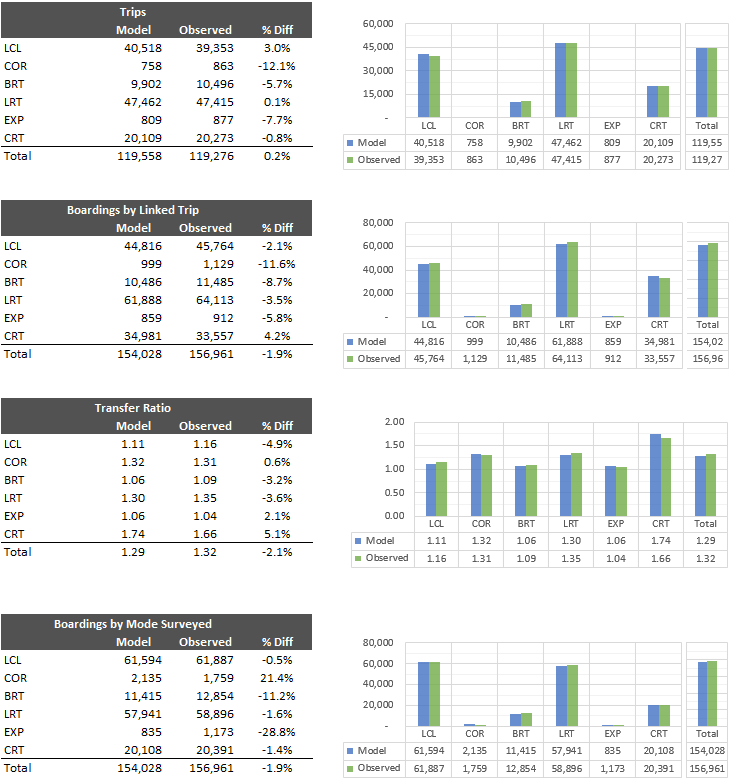
\includegraphics{v9x/v900/validation/_pictures/6-plot1.png}

}

\caption{\label{fig-pdf-boardings}Mode Choice boardings.}

\end{figure}

\hypertarget{mode-share-1}{%
\section{Mode Share}\label{mode-share-1}}

Figure~\ref{fig-pdf-trips-dy}, Figure~\ref{fig-pdf-trips-pk}, and
Figure~\ref{fig-pdf-trips-ok} show validation charts by modes, periods,
and purposes.

\begin{figure}[H]

{\centering 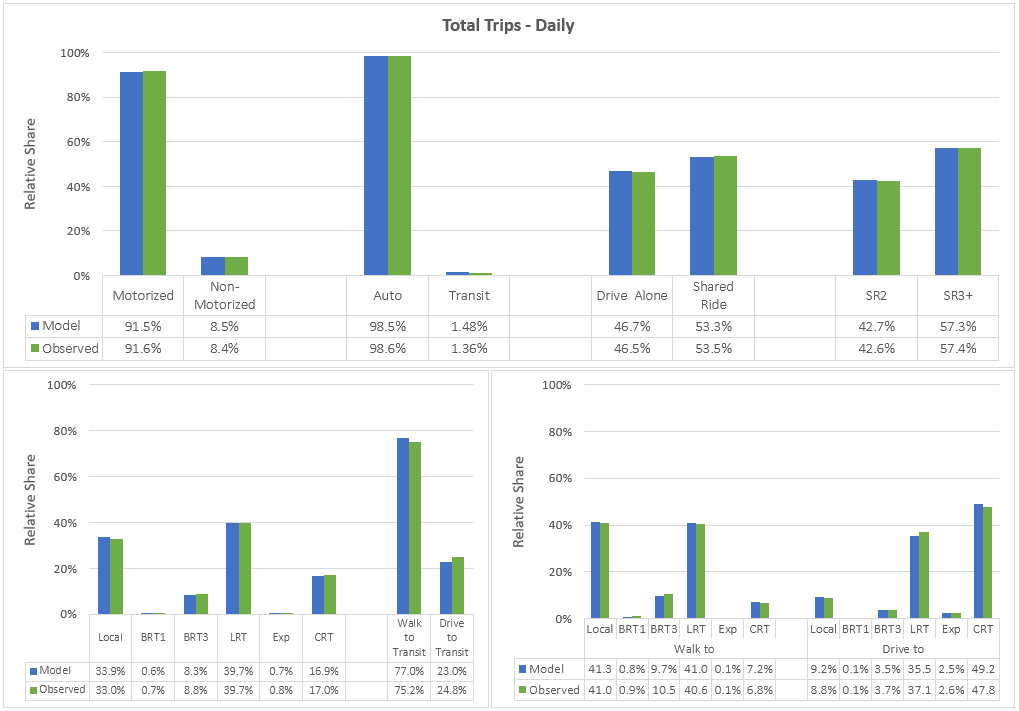
\includegraphics{v9x/v900/validation/_pictures/6-plot2.png}

}

\caption{\label{fig-pdf-trips-dy}Total Trips - Daily.}

\end{figure}

\begin{figure}[H]

{\centering 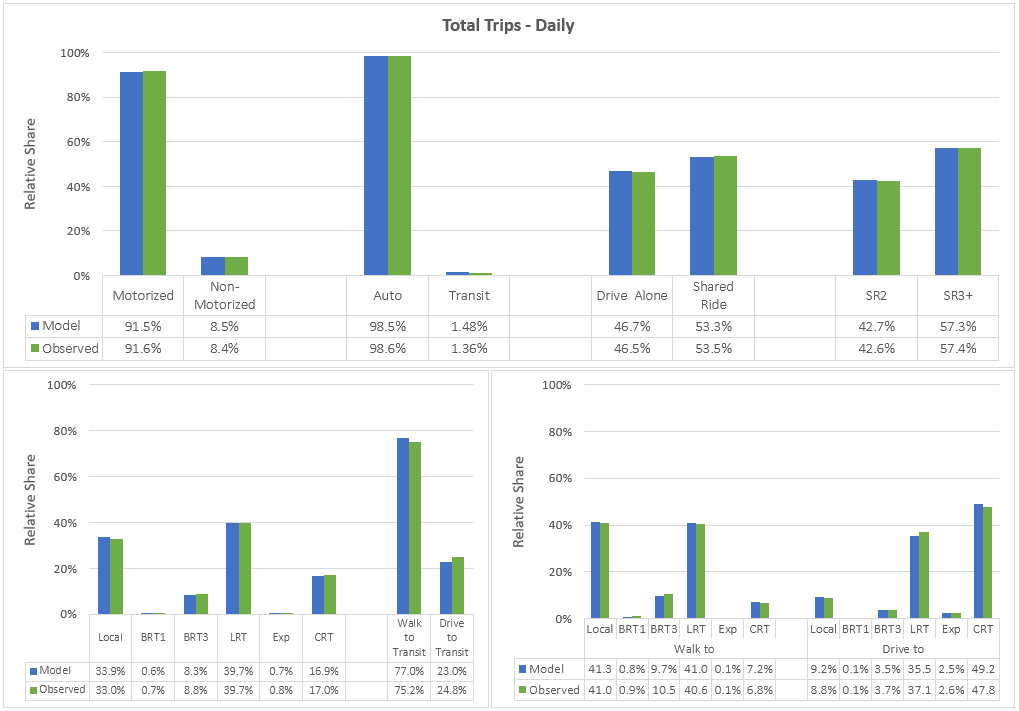
\includegraphics{v9x/v900/validation/_pictures/6-plot2.png}

}

\caption{\label{fig-pdf-trips-pk}Total Trips - Daily.}

\end{figure}

\begin{figure}[H]

{\centering 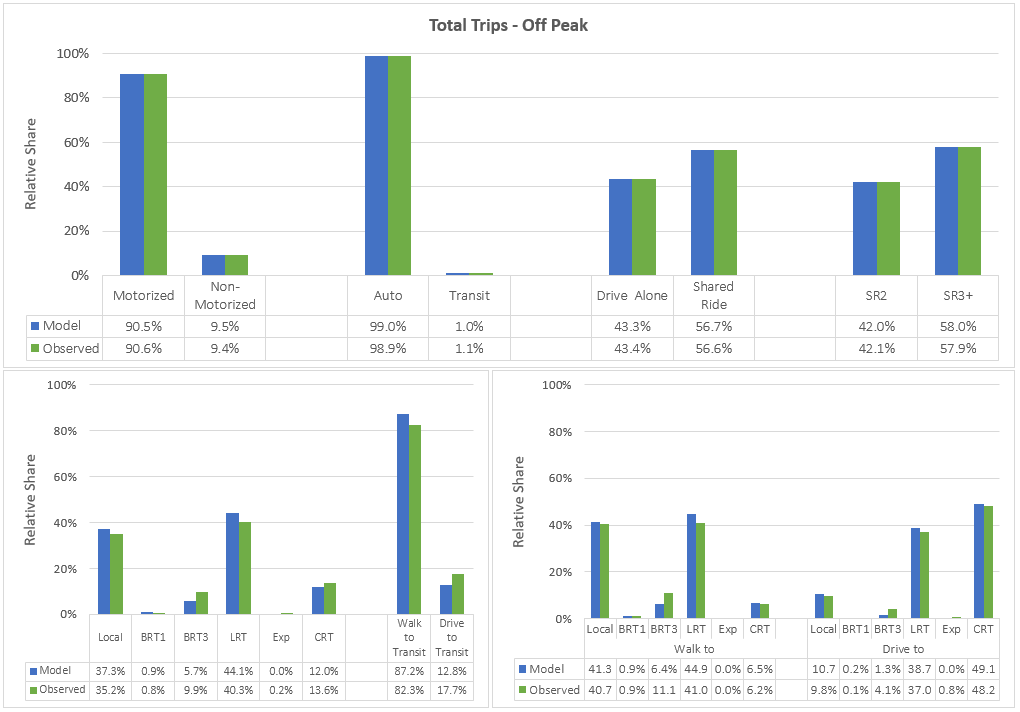
\includegraphics{v9x/v900/validation/_pictures/6-plot4.png}

}

\caption{\label{fig-pdf-trips-ok}Total Trips - Daily.}

\end{figure}

\bookmarksetup{startatroot}

\hypertarget{highway-assignment}{%
\chapter{Highway Assignment}\label{highway-assignment}}

The validation results for the Highway Assignment portion of the model
are shown in this section.The observed data for 2019 volumes is taken
from the Utah Department of Transportation (UDOT)
\href{https://drive.google.com/file/d/1rDXm0ObugGR1zXgWUuVbzWHNt-Xs1xru/view}{Average
Annual Daily Traffic (AADT) History} and associated with their
respective model segments. The traffic model data is taken from segment
summary report for the 2019 base year model:
\texttt{v9\_SE19\_Net19\_Summary\_SEGID.csv}. The results are divided
into three sections:

\begin{itemize}
\tightlist
\item
  Summary Comparison
\item
  Detailed Comparison
\item
  Map Comparison
\end{itemize}

\begin{Shaded}
\begin{Highlighting}[]
\NormalTok{import \{GroupedBarChart\} from "@d3/grouped{-}bar{-}chart"}
\NormalTok{import \{Legend, Swatches\} from "@d3/color{-}legend"}
\NormalTok{import \{howto, altplot\} from "@d3/example{-}components"}
\end{Highlighting}
\end{Shaded}

\begin{verbatim}
<IPython.core.display.HTML object>
\end{verbatim}

\begin{verbatim}
<IPython.core.display.HTML object>
\end{verbatim}

\begin{verbatim}
<IPython.core.display.HTML object>
\end{verbatim}

\begin{verbatim}
<IPython.core.display.HTML object>
\end{verbatim}

\begin{verbatim}
<IPython.core.display.HTML object>
\end{verbatim}

\begin{verbatim}
<IPython.core.display.HTML object>
\end{verbatim}

\begin{verbatim}
<IPython.core.display.HTML object>
\end{verbatim}

\begin{verbatim}
<IPython.core.display.HTML object>
\end{verbatim}

\begin{verbatim}
<IPython.core.display.HTML object>
\end{verbatim}

\begin{verbatim}
<IPython.core.display.HTML object>
\end{verbatim}

\begin{verbatim}
<IPython.core.display.HTML object>
\end{verbatim}

\begin{verbatim}
<IPython.core.display.HTML object>
\end{verbatim}

\begin{verbatim}
<IPython.core.display.HTML object>
\end{verbatim}

\begin{verbatim}
<IPython.core.display.HTML object>
\end{verbatim}

\begin{verbatim}
<IPython.core.display.HTML object>
\end{verbatim}

\hypertarget{summary-comparison}{%
\section{Summary Comparison}\label{summary-comparison}}

The summary comparison shows region and county-wide differences between
model and observed for \emph{Average Daily Volume} and
\emph{Vehicle-Miles Traveled (VMT)} by vehicle type. The values for Box
Elder and Weber counties are only the portions within the MPO planning
area. Validation was checked comparing the average daily volume at the
region and county levels. \textbf{?@fig-assign-summary}, below, contains
an interactive view of model vs observed differences by roadway class
and vehicle type.

\begin{Shaded}
\begin{Highlighting}[]
\NormalTok{html\textasciigrave{}\textless{}br/\textgreater{}\textasciigrave{}}
\NormalTok{viewof bSummaryFuncClass = Inputs.select(new Map([[\textquotesingle{}All Roadways\textquotesingle{},\textquotesingle{}All Roadways\textquotesingle{}], [\textquotesingle{}Freeway\textquotesingle{},\textquotesingle{}Freeway\textquotesingle{}], [\textquotesingle{}Principal\textquotesingle{},\textquotesingle{}Principal\textquotesingle{}], [\textquotesingle{}Minor\textquotesingle{}, \textquotesingle{}Minor\textquotesingle{}], [\textquotesingle{}Collector\textquotesingle{}, \textquotesingle{}Collector\textquotesingle{}]]), \{value: \textquotesingle{}All Roadways\textquotesingle{}, label: "Roadway Class:"\})}
\NormalTok{viewof bSummaryVehType = Inputs.select(new Map([[\textquotesingle{}All Vehicles\textquotesingle{},\textquotesingle{}All Vehicles\textquotesingle{}], [\textquotesingle{}Passenger Cars\textquotesingle{}, \textquotesingle{}Passenger Cars\textquotesingle{}], [\textquotesingle{}Medium Trucks\textquotesingle{},\textquotesingle{}Medium Trucks\textquotesingle{}], [\textquotesingle{}Heavy Trucks\textquotesingle{},\textquotesingle{}Heavy Trucks\textquotesingle{}]]), \{value: \textquotesingle{}All Vehicles\textquotesingle{}, label: "Vehicle Type:"\})}
\NormalTok{viewof bSummaryDiffType = Inputs.select(new Map([[\textquotesingle{}Percent Difference\textquotesingle{},\textquotesingle{}DiffPct\textquotesingle{}], [\textquotesingle{}Difference\textquotesingle{},\textquotesingle{}Diff\textquotesingle{}]]), \{value: \textquotesingle{}DiffPct\textquotesingle{}, label: "Display:"\})}
\end{Highlighting}
\end{Shaded}

\begin{Shaded}
\begin{Highlighting}[]

\NormalTok{volDiffLongT = transpose(volDiffLong)}
\NormalTok{vmtDiffLongT = transpose(vmtDiffLong)}

\NormalTok{volDiffLongT\_filtered = volDiffLongT.filter(function(dataL) \{}
\NormalTok{    return bSummaryFuncClass == dataL.funcClass \&\&}
\NormalTok{           bSummaryVehType == dataL.vehType \&\&}
\NormalTok{           ((\textquotesingle{}vol\textquotesingle{} + bSummaryDiffType) == dataL.View);}
\NormalTok{\})}
\NormalTok{vmtDiffLongT\_filtered = vmtDiffLongT.filter(function(dataL) \{}
\NormalTok{    return bSummaryFuncClass == dataL.funcClass \&\&}
\NormalTok{           bSummaryVehType == dataL.vehType \&\&}
\NormalTok{           ((\textquotesingle{}vmt\textquotesingle{} + bSummaryDiffType) == dataL.View);}
\NormalTok{\})}

\NormalTok{vvp = transpose(vvpct)}
\NormalTok{vvpL = transpose(vvpctLong)}
\NormalTok{vvaL = transpose(vvabsLong)}
\NormalTok{vvaLR = transpose(vvabsLongR)}
\end{Highlighting}
\end{Shaded}

\begin{Shaded}
\begin{Highlighting}[]
\NormalTok{//https://observablehq.com/@d3/diverging{-}bar{-}chart}
\NormalTok{import \{DivergingBarChart\} from "@d3/diverging{-}bar{-}chart"}

\NormalTok{function getXDomainVol(bSummaryDiffType) \{}
\NormalTok{    if (bSummaryDiffType === "Diff") \{}
\NormalTok{        return [max\_abs\_value\_volDiff * {-}1, max\_abs\_value\_volDiff];}
\NormalTok{    \} else \{}
\NormalTok{        return [max\_abs\_value\_volDiffPct * {-}1, max\_abs\_value\_volDiff]; // {-}100\% to 100\%}
\NormalTok{    \}}
\NormalTok{\}}

\NormalTok{function getXDomainVmt(bSummaryDiffType) \{}
\NormalTok{    if (bSummaryDiffType === "Diff") \{}
\NormalTok{        return [max\_abs\_value\_vmtDiff * {-}1, max\_abs\_value\_vmtDiff];}
\NormalTok{    \} else \{}
\NormalTok{        return [max\_abs\_value\_vmtDiffPct * {-}1, max\_abs\_value\_vmtDiff]; // {-}100\% to 100\%}
\NormalTok{    \}}
\NormalTok{\}}
\end{Highlighting}
\end{Shaded}

\begin{Shaded}
\begin{Highlighting}[]
\NormalTok{html\textasciigrave{}\textless{}br/\textgreater{}\textless{}h4\textgreater{}Average Daily Volume\textless{}/h4\textgreater{}\textasciigrave{}}
\NormalTok{chartVolDiff = DivergingBarChart(volDiffLongT\_filtered, \{}
\NormalTok{    x: d =\textgreater{} d.ViewValue,}
\NormalTok{    y: d =\textgreater{} d.coFips,}
\NormalTok{    xFormat: bSummaryDiffType === "Diff" ? "+,d" : "+.1\%",}
\NormalTok{    xLabel: "Model vs Observed Differences",}
\NormalTok{    width: 440,}
\NormalTok{    xDomain: bSummaryDiffType === "Diff" ? [max\_abs\_value\_volDiff * {-}1, max\_abs\_value\_volDiff] : [max\_abs\_value\_volDiffPct * {-}1, max\_abs\_value\_volDiffPct],}
\NormalTok{    yDomain:  [\textquotesingle{}Region\textquotesingle{},\textquotesingle{}Box Elder County {-} WFRC\textquotesingle{},\textquotesingle{}Weber County {-} WFRC\textquotesingle{},\textquotesingle{}Davis County\textquotesingle{},\textquotesingle{}Salt Lake County\textquotesingle{},\textquotesingle{}Utah County\textquotesingle{}],}
\NormalTok{    colors: d3.schemeRdBu[3]}
\NormalTok{\})}
\end{Highlighting}
\end{Shaded}

\begin{Shaded}
\begin{Highlighting}[]
\NormalTok{html\textasciigrave{}\textless{}br/\textgreater{}\textless{}h4\textgreater{}Vehicle{-}Miles Traveled\textless{}/h4\textgreater{}\textasciigrave{}}
\NormalTok{chartVmtDiff = DivergingBarChart(vmtDiffLongT\_filtered, \{}
\NormalTok{    x: d =\textgreater{} d.ViewValue,}
\NormalTok{    y: d =\textgreater{} d.coFips,}
\NormalTok{    xFormat: bSummaryDiffType === "Diff" ? "+,d" : "+.1\%",}
\NormalTok{    xLabel: "Model vs Observed Differences",}
\NormalTok{    width: 440,}
\NormalTok{    xDomain: bSummaryDiffType === "Diff" ? [max\_abs\_value\_vmtDiff * {-}1, max\_abs\_value\_vmtDiff] : [max\_abs\_value\_vmtDiffPct * {-}1, max\_abs\_value\_vmtDiffPct],}
\NormalTok{    yDomain:  [\textquotesingle{}Region\textquotesingle{},\textquotesingle{}Box Elder County {-} WFRC\textquotesingle{},\textquotesingle{}Weber County {-} WFRC\textquotesingle{},\textquotesingle{}Davis County\textquotesingle{},\textquotesingle{}Salt Lake County\textquotesingle{},\textquotesingle{}Utah County\textquotesingle{}],}
\NormalTok{    colors: d3.schemeRdBu[3]}
\NormalTok{\})}
\end{Highlighting}
\end{Shaded}

\begin{Shaded}
\begin{Highlighting}[]
\NormalTok{//|label: fig{-}assign{-}summary}
\NormalTok{//|fig{-}cap: Highway Assignment Summary Comparison}
\NormalTok{tbEmptyCell1 = 1}
\end{Highlighting}
\end{Shaded}

At the region level model volume is 0.2\% lower than observed volume.
The four more urban counties (Weber, Davis, Salt Lake, and Davis) were
all within 5\% of observed volumes with Salt Lake County being the
closest. Weber and Davis were slightly lower and Utah County was
slightly higher. Box Elder County is more rural than the other counties.
Box Elder model volumes are about 10\% lower than observed. Time did not
allow for further calibration of the volumes in Box Elder area to
account for the larger differences.

One important observation at the \emph{Collector} and \emph{All
Vehicles} level is that Utah County shows a much higher difference than
the other counties. Upon further investigation of observed
\emph{Collector} volumes in Utah County, many roadway segments had very
low volumes compared to what was expected. Utah County is one of the
highest growth areas in the region. For this reason, we expect that the
observed count data may be underrepresenting actual volumes. We also
anticipate observed volumes in Utah County to improve in the near-term.
Within the last several years, a large investment in continuous count
station in Utah County has been made. The new counters will add
additional information to generate observed volumes for all roadway
segments.

The largest differences in model vs observed volumes occur in the Medium
Truck and Heavy Truck vehicle types. A good amount of time was spent
attempting to bring model truck volumes closer to observed. However, due
to the limited data sources for truck information, further need to
investigate observed truck volumes, and a desire to not over-calibrate
the model, further calibration was stopped. Truck modeling remains a
future priority for model improvement.

\hypertarget{detailed-comparison}{%
\section{Detailed Comparison}\label{detailed-comparison}}

The model vs observed details in this section are presented by volume
and Vehicle-Miles Traveled (VMT) through the comparison of model and
observed data facility type by region and also by county.
\textbf{?@fig-assign-validation} allows for the interactive visual
comparison of model and observed values for the region and each county
for all vehicles, cars, medium trucks, and heavy trucks. The comparisons
are shown in four different types of charts and tables:

\begin{itemize}
\tightlist
\item
  \emph{Average Daily Volume by Roadway Class (2a)}: The daily volume is
  averaged across all segments within their respective geography and
  vehicle type.
\item
  \emph{Total VMT by Roadway Class (2b)}: For each segment*, the daily
  volume is multiplied by segment distance and then summed across all
  segments within their respective geography and vehicle type.
\item
  \emph{Model vs Count Segment Volume (2c)}: This is a scatter plot of
  segment daily volume with the x-axis as the observed volume and the
  y-axis as the model volume. The red line shows the location of where
  model and observed volumes are equal. The dashed blue line shows a
  least-squares linear regression. The further the blue line moved away
  from the red line, the further the model is from observed.
\item
  \emph{Segment Percent Error (2d)}: This is a scatter plot showing the
  amount of error (percent difference) between the observed volume and
  the model volume. The observed volume is the x-axis and the percent
  error is the y-axis. The red lines are a bounding box that shows the
  control target. As volume increases, it is expected that the percent
  error should decrease.
\end{itemize}

\begin{figure}[H]

{\centering 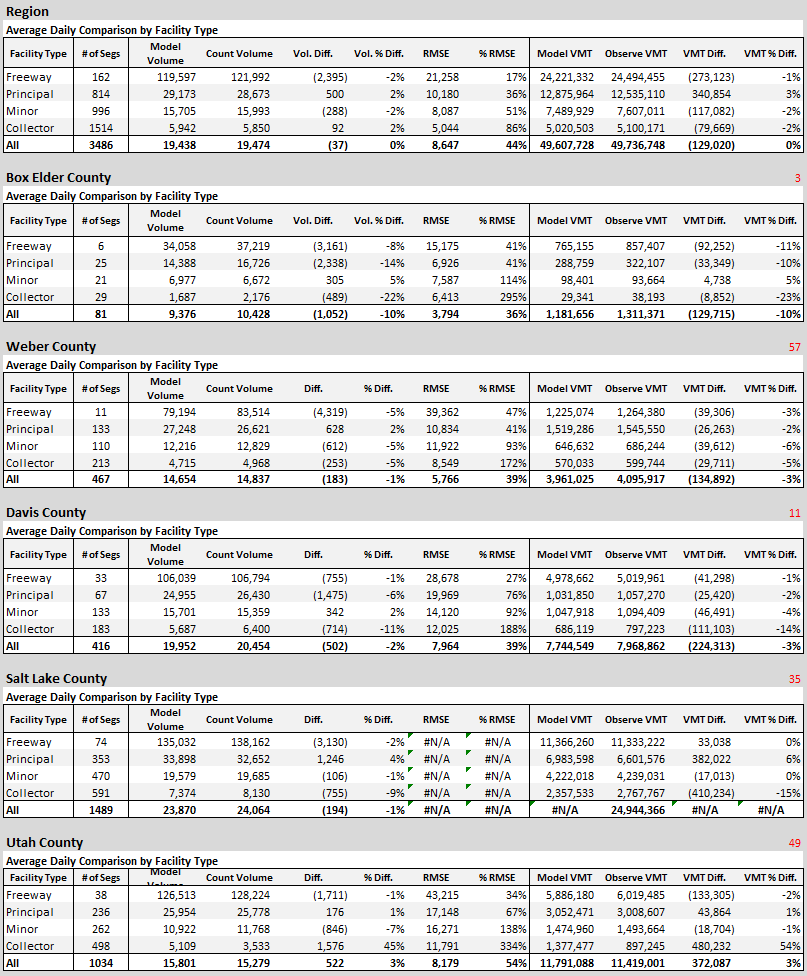
\includegraphics{v9x/v900/validation/_pictures/7-plot1.png}

}

\caption{\label{fig-pdf-ave-ft}Average Daily Comparison by Facility Type
by Region.}

\end{figure}

\hypertarget{validation-charts}{%
\section{Validation Charts}\label{validation-charts}}

Write some words here.

\begin{figure}[H]

{\centering 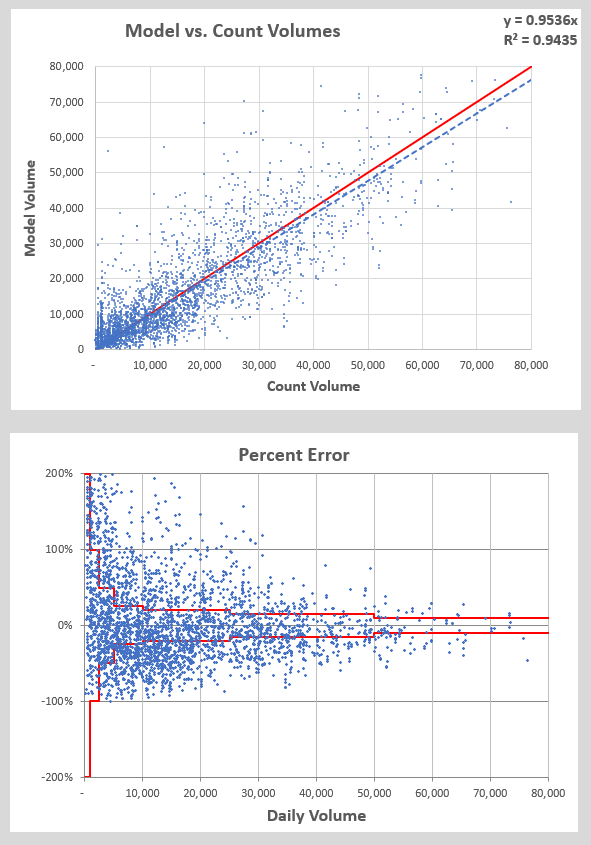
\includegraphics[width=\textwidth,height=0.6\textheight]{v9x/v900/validation/_pictures/7-plot2.png}

}

\caption{\label{fig-allvehicles}Volume Comparison -- All Vehicles.}

\end{figure}

\begin{figure}[H]

{\centering 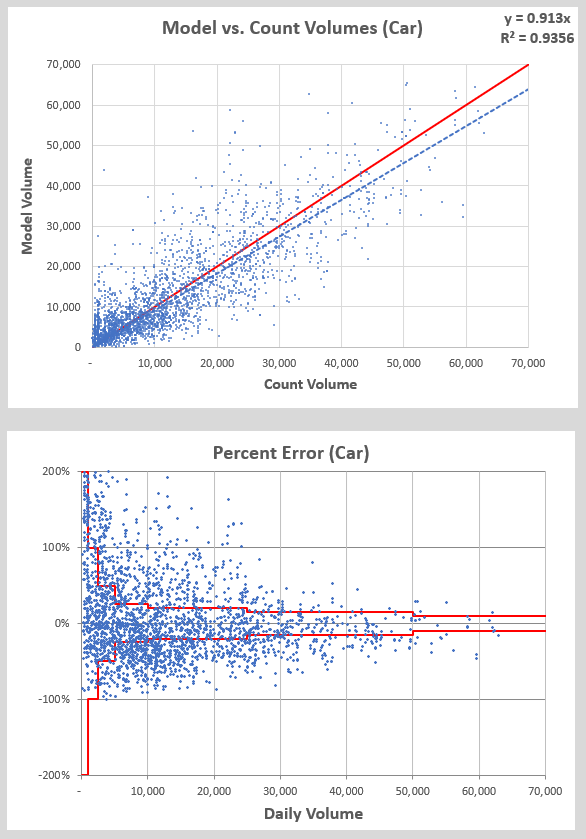
\includegraphics[width=\textwidth,height=0.6\textheight]{v9x/v900/validation/_pictures/7-plot3.png}

}

\caption{\label{fig-pc}Volume Comparison -- Passenger Cars.}

\end{figure}

\begin{figure}[H]

{\centering 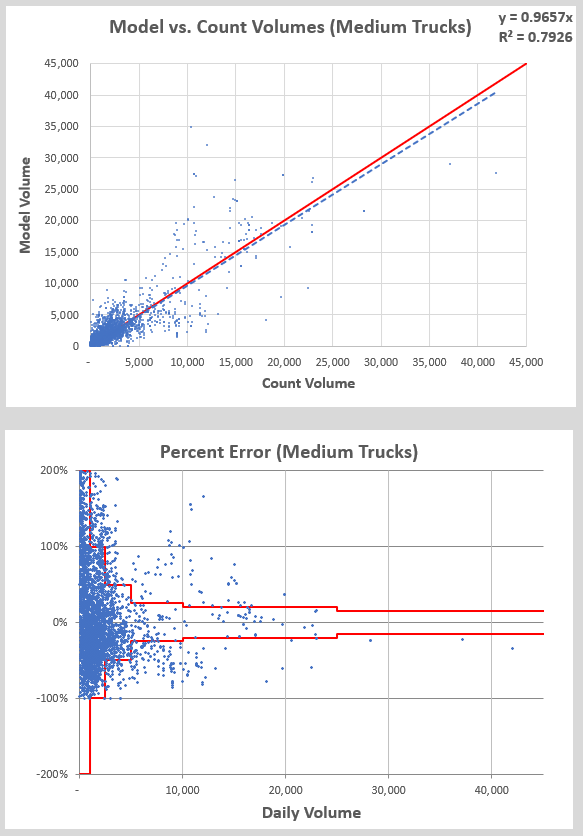
\includegraphics[width=\textwidth,height=0.6\textheight]{v9x/v900/validation/_pictures/7-plot4.png}

}

\caption{\label{fig-md-trucks}Volume Comparison -- Medium Trucks.}

\end{figure}

\begin{figure}[H]

{\centering 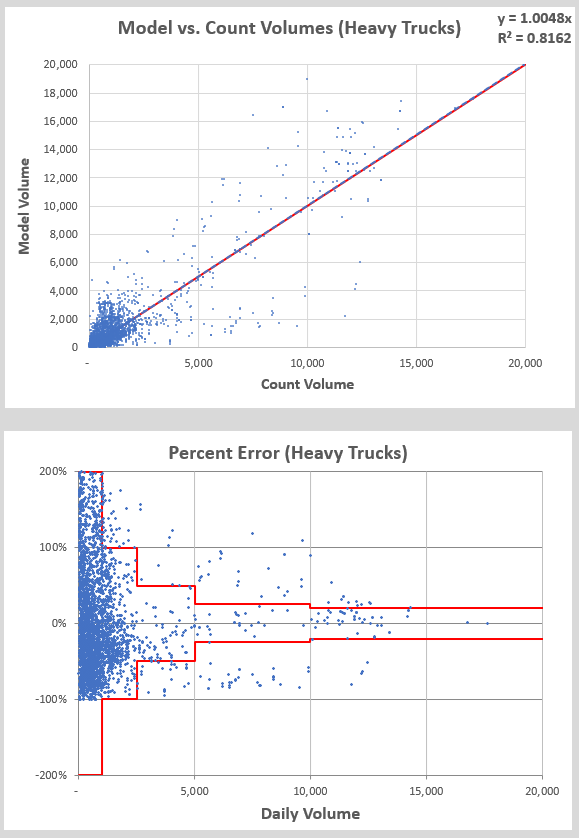
\includegraphics[width=\textwidth,height=0.6\textheight]{v9x/v900/validation/_pictures/7-plot5.png}

}

\caption{\label{fig-hv-trucks}Volume Comparison -- Heavy Trucks.}

\end{figure}

\hypertarget{map-comparison}{%
\section{Map Comparison}\label{map-comparison}}

The maps in Figure~\ref{fig-map} shows a comparison of segment level
model vs observed volumes by vehicle types. Blue represents model lower
than observed and red represent model volume higher than observed.

\begin{figure}[H]

{\centering 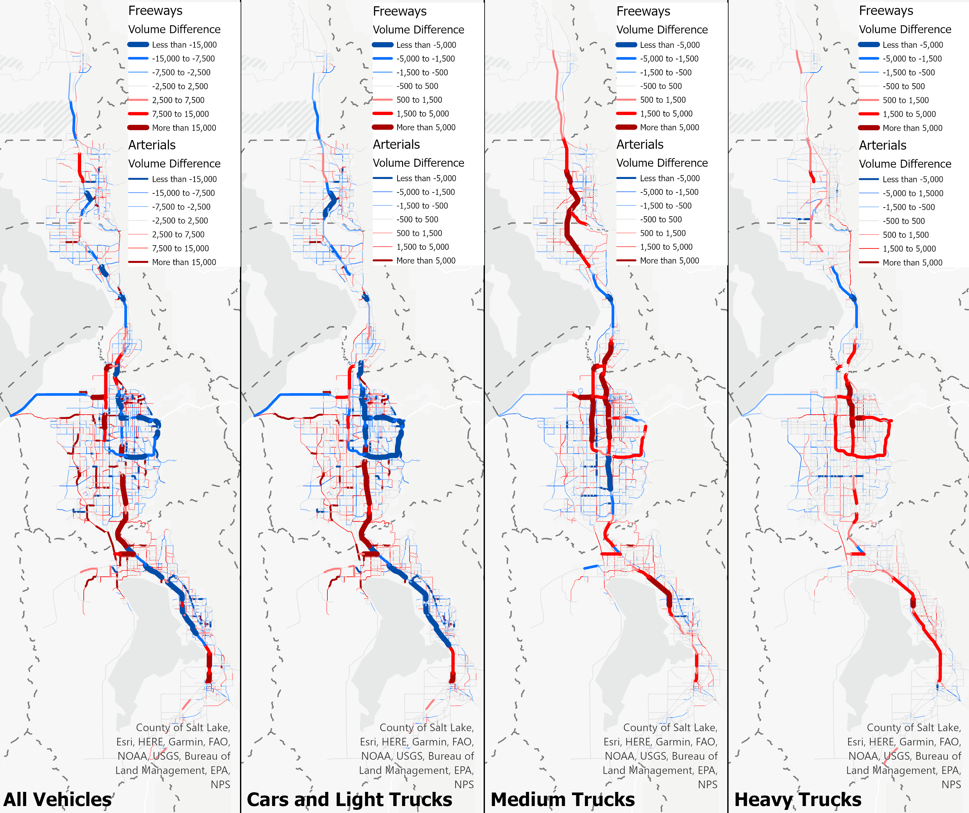
\includegraphics{v9x/v900/validation/_pictures/7-plot6.png}

}

\caption{\label{fig-map}Segment-Level Model vs Observed Volume
Comparison by Vehicle Type}

\end{figure}

Looking at the \emph{All Vehicles} map, the model volumes are lower than
observed for by more than 15,000 vehicles per day for the east side of
I-215 and for I-15 through northern Utah County. Model volumes are
higher than observed volumes by more than than 15,000 vehicles for I-15
in southern Salt lake County and for I-15 in Utah County between
Springville and Spanish Fork. When looking at these areas by vehicle
type, the drop in \emph{Cars and Light Trucks} are actual greater since
the \emph{Medium Trucks} and \emph{Heavy Trucks} in these areas are
greater in the model vs observed. Outside of these areas, the volume
differences between model and observed are relatively minor.

The lower arterial model vs observed volumes of \emph{Heavy Trucks} on
9000 South in Salt Lake County was further investigated. The \emph{Heavy
Truck} observed volume for this roadway seemed much higher than expected
for this roadway. The lower volumes are likely due to the observed data
and not anything in the model.

\bookmarksetup{startatroot}

\hypertarget{sensitivity-tests}{%
\chapter{Sensitivity Tests}\label{sensitivity-tests}}

???Did we do any sensitivity tests???



\end{document}
